\documentclass[12pt, a4paper]{article}
\usepackage{import}
\usepackage{preamble}

\title{Regression and Curve Fitting}
\date{6\(^\text{{th}}\) October 2022}
\author{Lee Farrugia}

\begin{document}
    
\maketitle
\thispagestyle{titlepagestyle}
\pagestyle{mystyle}

\section{Task 1 - Simple Linear Regression}

\subsection{Introduction and Theoretical Background}
The generic term ``Regression'' in the case of statistical methods is the attempt to fit a model to the data in order to determine the relationship between the outcome and input data. Regression can be done using different methods, one of which, ordinary least squares, was used in this task.

Specifically for this task the data for a Young's Modulus experiment was fitted with the use of the ordinary least squares regression in order to obtain the straight line graph. The ordinary least squares method was applied on the data by the use of python. The input data was obtained through an experiment of Young's Modulus, which was done by varying weights applied to a tinned copper wire and measuring the resultant depression of the contact point.

\subsection{Materials and Methods}

\subsubsection{Languages and Packages}
Python 3.10.8, Pandas, Numpy, Matplolib.pyplot.

\subsubsection{Methodology}
\begin{enumerate}
    \item The dataset provided was imported into the program, each variable defined according to its respective column of data, and each variable was converted into an array with the use of numpy.
    \item A function was constructed to calculate the \(\alpha\) and \(\beta\) that correspond to the \(\alpha\) and \(\beta\) of the equation:
    \begin{equation}
        \label{equation 1}\\
        Y_e = \alpha + \beta X\,.
    \end{equation}
    \(\alpha\) and \(\beta\) were further defined as the following:
    \begin{align}
        \label{equation 2}\\
        \beta &= \frac{\sum_{i=1}^{n}(X_i - \bar{X})(Y_i - \bar{Y})}{\sum_{i=1}^{n}(X_i - \bar{X})^2} ,\\
        \label{equation 3}
        \alpha &= \bar{Y} - \beta \bar{X} .
    \end{align}
    \item This function was further expanded to include the calculation of the uncertainties of \(\alpha\) and \(\beta\), and the correlation coefficient and coefficient of determination.
    \item Using this function the experimental values for \(E\) and \(T_0\) and their respective uncertainties were calculated. Using these values a trendline was generated, with the residuals being plotted directly underneath it. 
\end{enumerate}

\subsection{Results}
\begin{longtable}{|c|c|c|c|c|c|}
\hline \(\beta\) & \(\Delta \beta\) & \(\alpha\) & \(\Delta \alpha\) & r & R\\ \hline
\endfirsthead

\hline \(\beta\) & \(\Delta \beta\) & \(\alpha\) & \(\Delta \alpha\) & r & R\\ \hline
\endhead

1266912.35 & 81009.26 & 12.51 & 0.67 & 0.99 & 0.99\\ \hline

\caption{Table of Function Results}
\label{tab: Table 1.1}\\
\end{longtable}

\begin{longtable}{|c|c|c|c|}
\hline Gradient/Nm\(^2\) & \(\Delta\)Gradient/Nm\(^2\)  & Intercept/Nm\(^2\) & \(\Delta\)Intercept/Nm\(^2\)\\ \hline
\endfirsthead

\hline Gradient/Nm\(^2\) & \(\Delta\)Gradient/Nm\(^2\)  & Intercept/Nm\(^2\) & \(\Delta\)Intercept/Nm\(^2\)\\ \hline
\endhead

1266912.35 & \SI{4.67e-10}{} & 12.51 & \SI{3.84e-15}{} \\ \hline

\caption{Table of Results from the Graph}
\label{tab: Table 1.2}\\
\end{longtable}

\begin{longtable}{|c|c|c|c|}
\hline E/Nm\(^2\) &\(\Delta\)E/Nm\(^2\) & \(\text{T}_0\)/N & \(\Delta\)\(\text{T}_0\)/N\\ \hline
\endfirsthead

\hline E/Nm\(^2\) & \(\Delta\)E/Nm\(^2\) & \(\text{T}_0\)/N & \(\Delta\)\(\text{T}_0\)/N\\ \hline
\endhead

\SI{2.79e11}{} & \SI{101}{} & \SI{7.98}{} & \SI{0.03}{}\\ \hline

\caption{Results of Young's Modulus and Initial tension}
\label{tab: Table 1.3}\\
\end{longtable}

\begin{table}[H]
\centering
\begin{tabular}{|c|c|c|c|c|c|}
\hline
Residuals & -0.36 & -0.11 & 0.48 & 0.72 & -0.73 \\\hline
\end{tabular}
\caption{Table of Residuals}
\label{tab: Table 1.4}
\end{table}

\subsection{Discussion}
In order to calculate \(\alpha\) and \(\beta\), a function was created to match equation~\ref{equation 2}. Additionally, the function was expanded to also calculate the correlation and determination coefficients. This can be seen in the following piece of code:
\begin{minted}{py}
def beta_alpha_function(xi, xbar, yi, ybar):
    for i in range(len(xi)):
        prod = (xi[i]-xbar)*(yi[i]-ybar)
        prodlist.append(prod)
        xdenom = (xi[i]-xbar)**2
        denomlist.append(xdenom)
        ydenom = (yi[i]-ybar)**2
        ydenomlist.append(ydenom)
    prod_array = np.array(prodlist)
    denom_array = np.array(denomlist)
    ydenom_array = np.array(ydenomlist)
    numerator = sum(prod_array)
    denominator = sum(denom_array)
    ydenominator = sum(ydenom_array)
    beta = numerator/denominator
    alpha = ybar - (beta*xbar)
    r = numerator/(np.sqrt(denominator*ydenominator))
    delta_beta = (beta/(np.sqrt(len(xi)-2)))*(np.sqrt((1/r**2)-1))
    delta_alpha = delta_beta*np.sqrt(((1/len(xi))*(sum(xi**2))))
    R = r**2
    return beta, alpha, delta_beta, delta_alpha, r, R .
\end{minted}
The values for \(\alpha\) and \(\beta\) were then used to plot the fit for the data given and obtain the Young's Modulus of the wire and its initial tension. The fit resulted in a straight line were the Young's Modulus was the gradient and the initial tension was the y-intercept. This can be further seen from the obtain figure~\ref{fig:Fig 1.1}. Furthermore, the residuals of the the points to the fit were also calculated using by finding the difference of the original data point and the fitted data points and these were plotted underneath the original straight line plot. 

\subsection{Figures and Graphs}
\begin{figure}[H]
    \centering
    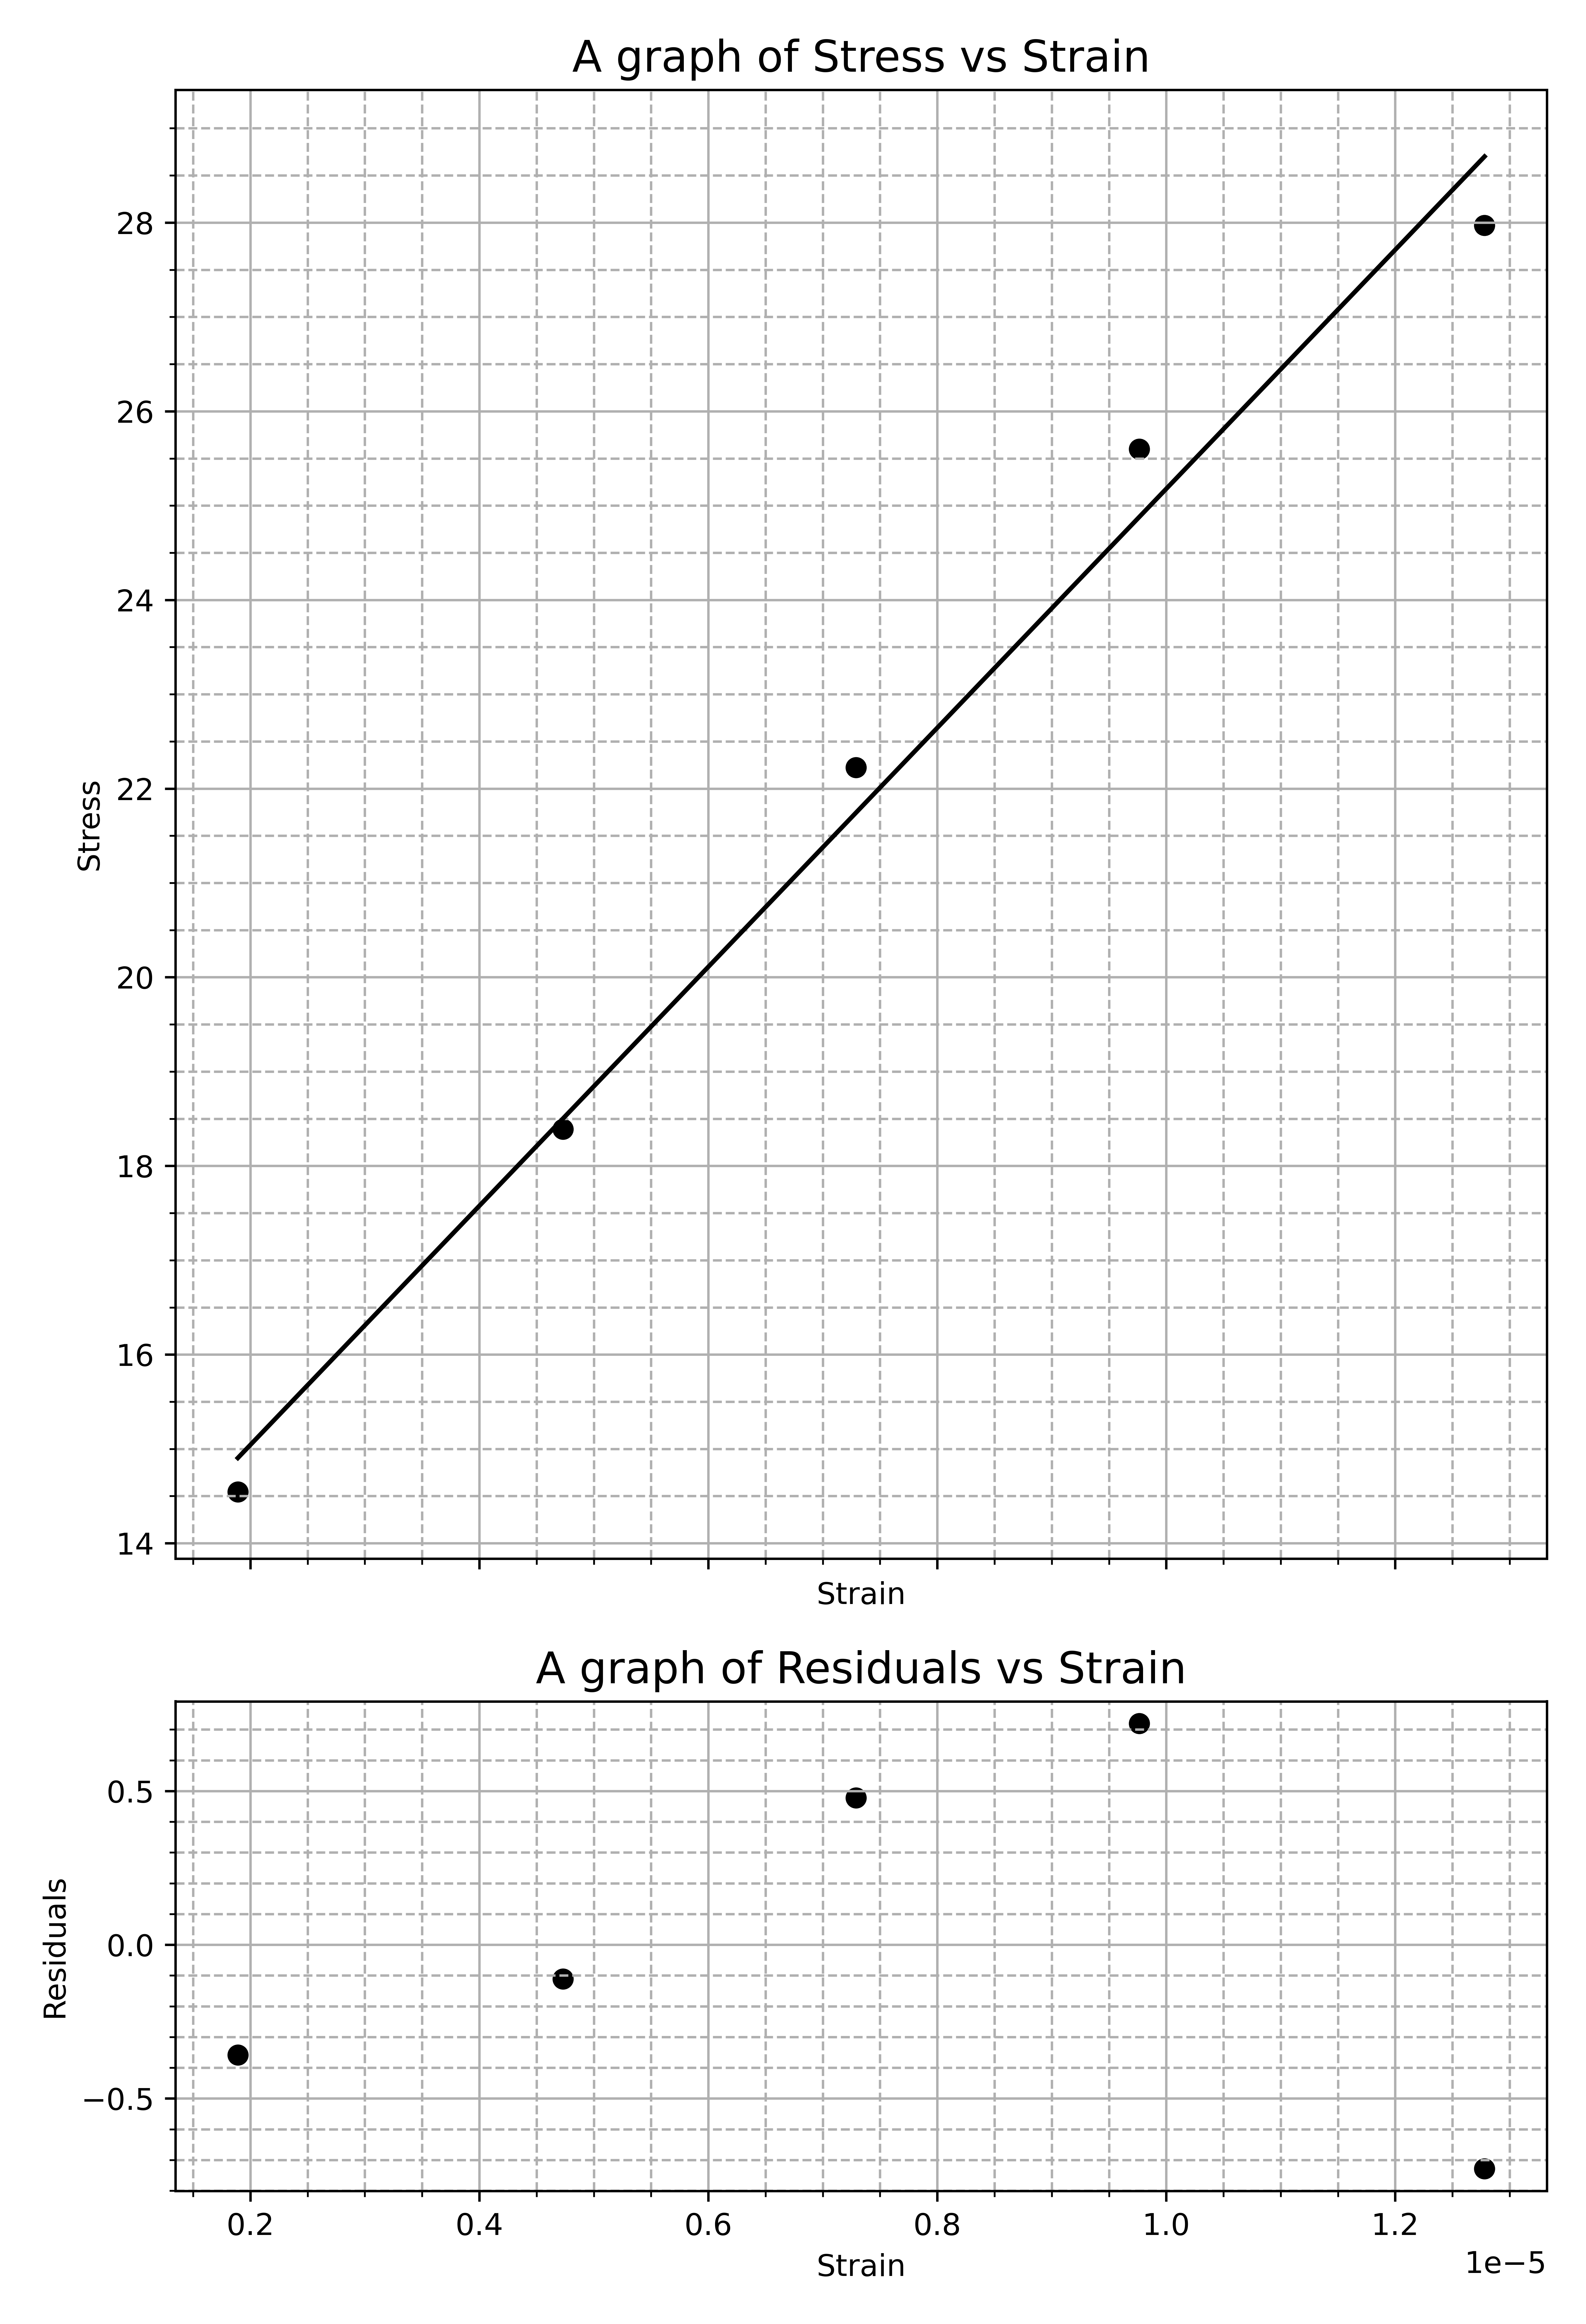
\includegraphics[width = \textwidth]{1Plot1.png}
    \caption{A graph of stress vs strain and their respective residuals}
    \label{fig:Fig 1.1}
\end{figure}

\subsection{Appendix}
\begin{minted}{py}
# Task 1

import numpy as np
import pandas as pd
import matplotlib.pyplot as plt

# creating the empty lists to be used
xlist = []
ylist = []
prodlist = []
denomlist = []
ydenomlist = []
yelist = []

# reading the data
data = pd.read_csv('Q1__Youngs_Modulus_of_a_Wire.csv')
# changing the individual columns into arrays
diameter_array = (data['Diameter/m']).to_numpy()
mass_array = data['m/kg'].to_numpy()
x1_array = data['x_1/m'].to_numpy()
x2_array = data['x_2/m'].to_numpy()
x3_array = data['x_3/m'].to_numpy()
x4_array = data['x_4/m'].to_numpy()
L_array = data['L/m'].to_numpy()
x0_array = data['x_0/m'].to_numpy()

# finding the x-x0 part of the equation
for i in range(len(x1_array)-1):
    x = sum([x1_array[i], x2_array[i], x3_array[i], x4_array[i]])
    X = (x/4)-x0_array[0]
    xlist.append(abs(X))

# calculating xi and xbar
xi = np.array(xlist)**2
xbar = np.mean(xi)

# calculating yi and y bar
for i in range(len(mass_array)-1):
    yi = mass_array[i]/xlist[i]
    ylist.append(yi)

yi = np.array(ylist)
ybar = np.mean(yi)

# defining the function to calculate alpha, beta, coefficient of correlation and determination
def beta_alpha_function(xi, xbar, yi, ybar):
    for i in range(len(xi)):
        prod = (xi[i]-xbar)*(yi[i]-ybar)
        prodlist.append(prod)
        xdenom = (xi[i]-xbar)**2
        denomlist.append(xdenom)
        ydenom = (yi[i]-ybar)**2
        ydenomlist.append(ydenom)
    prod_array = np.array(prodlist)
    denom_array = np.array(denomlist)
    ydenom_array = np.array(ydenomlist)
    numerator = sum(prod_array)
    denominator = sum(denom_array)
    ydenominator = sum(ydenom_array)
    beta = numerator/denominator
    alpha = ybar - (beta*xbar)
    r = numerator/(np.sqrt(denominator*ydenominator))
    delta_beta = (beta/(np.sqrt(len(xi)-2)))*(np.sqrt((1/r**2)-1))
    delta_alpha = delta_beta*np.sqrt(((1/len(xi))*(sum(xi**2))))
    R = r**2
    return beta, alpha, delta_beta, delta_alpha, r, R

# calling previous function to get the actual values
beta, alpha, delta_beta, delta_alpha, r, R = beta_alpha_function(xi, xbar, yi, ybar)

# calculating the experimental values 
for i in range(len(xi)):
    ye = alpha + (beta*xi[i])
    yelist.append(ye)
ye_array = np.array(yelist)

# calculating the constants for the gradient and intercept
radius = np.average(diameter_array)
m_constant = (8*np.pi*(radius**2))/(9.81*(L_array[0]**3))
c_constant = 4/(L_array[0]*9.81)

# finding the line of best fit to the data
coeffs, cov = np.polyfit(xi, ye_array, 1, cov=True)
polyfunc = np.poly1d(coeffs)
trendline = polyfunc(xi)

# calculating the young's modulus and T0
E = coeffs[0]/m_constant
T0 = coeffs[1]/c_constant
grad_error = np.sqrt(cov[0][0])
inter_error = np.sqrt(cov[1][1])

g = 9.81

delta_E = np.sqrt(((((g*(L_array**3)) / (8*np.pi*(r**2))) * (grad_error))**2) + ((((3*(L_array**2) * coeffs[0]*g) / (8*np.pi*(r**2))) * (0.001))**2) + ((((-2*coeffs[0] * g * (L_array**3)) / (8*np.pi*(r**3)))*(1e-4))**2))
delta_T0 = np.sqrt(((((L_array*g)/4) * (inter_error))**2) + ((((coeffs[1]*g)/4) * (0.001))**2))

print(f'The value of E is : {E}, with an error of: {delta_E}. The value of T0: {T0}, with and error of {delta_T0}')

# calculating the residuals
residual = np.subtract(yi,trendline)

print(residual)

f, (a0, a1) = plt.subplots(2, 1, sharex=True, sharey=False, gridspec_kw={'height_ratios': [3, 1]}, figsize=(7.3, 10.7))

# defining the font to be used
plt.rcParams['font.family'] = 'STIXGeneral'
plt.rcParams['mathtext.fontset'] = 'stix'
plt.rcParams['font.size'] = 12
plt.rcParams['font.weight'] = 'normal'

# plotting both graph as subplots
a0.scatter(xi, yi, color='k', label='Data Points')
a0.plot(xi, trendline, color='k', label='Trendline')
a0.minorticks_on()
a0.grid(visible=True, which='major', linestyle='-')
a0.grid(visible=True, which='minor', linestyle='--')
a0.set_xlabel('Strain')
a0.set_ylabel('Stress')
a0.set_title('A graph of Stress vs Strain')

a1.scatter(xi, residual, color='k')
a1.minorticks_on()
a1.grid(visible=True, which='major', linestyle='-')
a1.grid(visible=True, which='minor', linestyle='--')
a1.set_ylabel('Residuals')
a1.set_xlabel('Strain')
a1.set_title('A graph of Residuals vs Strain')
f.tight_layout()
f.savefig('1Plot1.png', dpi=800)
f.show()

\end{minted}
\newpage

\section{Task 2 -  Polynomial Regression \& Power Law Fitting}

\subsection{Introduction and Theoretical Background}
Sometimes the relationship between the output variable and the predictor variable do not follow a linear relationship, thus the need arises to find a way to fit this relationship. This is achieved by using the Polynomial Regression. In this case rather than having the previous equation of:
\begin{equation}
    Y = \alpha + \beta X ,
\end{equation}
we now have the equation in the polynomial form of:
\begin{equation}
    Y = \theta_0 + \theta_1 x^1+ \theta_2 x^2 + \theta_3 x^3 + \cdots + \theta_n x^n .
\end{equation}
\(n\) in this case is the degree of the polynomial which when increases will increase the polynomial complexity but in certain cases this higher value is needed to fit accordingly.

In this task, we are asked to find the polynomial regression fit to the Hertzsprung-Russell Diagram. This plots the temperature of the starts in question against their luminosity, which allows us to characterise the individual stars and track how they evolve \parencite{muncaster}.

\subsection{Materials and Methods}
\subsubsection{Languages and Packages}
Python 3.10.8, Pandas, Numpy, Matplolib.pyplot, Scipy, sklearn.

\subsubsection{Methodology}
\begin{enumerate}
    \item The data was imported into the code, and it was split according to the stellar type and the relative luminosity was plotted against the temperature. 
    \item As the variance was too large, the logarithm of both plotting variables was taken in order to produce a better scale. 
    \item The data was then filtered to only consider the data for the ``Main sequence''.
    \item This data was fitted to the Stefan-Boltzmann power law, which is defined as: 
    \begin{equation} 
        f(x) = \alpha x^{\beta} ,
    \end{equation}
    which was adapted for the equation:
    \begin{equation}
        L = A \sigma T^4 .
    \end{equation}
    \item From the previous equation \(\sigma\) was calculated using the \mintinline{python}{curve_fit} function of \mintinline{python}{scipy}, and this value is then compared with the theoretical value. These values were then used to calculate the stellar radii of the star given in a second data set.
\end{enumerate}

\subsection{Results}
\begin{longtable}{|c|c|}
    \hline Polynomial Degree & Root Mean Square Error \\ \hline
    \endfirsthead

    \hline Polynomial Degree & Root Mean Square Error \\ \hline
    \endhead

    2 & 1.06954\\ \hline
    10 & 0.99632 \\ \hline
    15 & 0.99301 \\ \hline
    16 & 0.99286 \\ \hline
    17 & 0.99289 \\ \hline
    20 & 0.99396 \\ \hline
    30 & 1.00272 \\ \hline

    \caption{Table of Polynomial Degrees and Root Mean Square Errors}
    \label{Tab: Table 2.1}\\
\end{longtable}

\begin{table}[H]
    \centering
    \begin{tabular}{|c|c|}
        \hline 
        Experimental Boltzamnn constant & 5.89 \(\times\) 10\(^{-8}\) \\ \hline
        Theoretical Boltzmann constant & 5.67 \(\times\) 10\(^{-8}\) \\ \hline
        Accuracy & 3.85\% \\ \hline
    \end{tabular}
    \caption{Table of Boltzmann Values and the Accuracy}
    \label{Tab: Table 2.2}
\end{table}

\begin{longtable}{|c|c|c|c|c|c|}
    \hline Star & T/K & L/L\(_0\) & Theoretical Radius & Experimental Radius & Accuracy\\ \hline
    \endfirsthead

    \hline Star & T/K & L/L\(_0\) & Theoretical Radius & Experimental Radius & Accuracy\\ \hline
    \endhead

    Beltelgeuse (min) & 3600 & 90000 & 5.38 \(\times\) 10\(^{11}\) & 5.28 \(\times\) 10\(^{11}\) & 1.87\%\\ \hline
    Beltelgeuse (max) & 3600 & 150000 & 2.20 \(\times\) 10\(^{11}\) & 2.15 \(\times\) 10\(^{11}\) & 1.87\%\\ \hline
    Arcturus & 4286 & 170 & 1.65 \(\times\) 10\(^{10}\) & 1.62 \(\times\) 10\(^{10}\) & 1.85\%\\ \hline
    TRAPPIST-1.000000 & 2566 & 0.000553 & 8.30 \(\times\) 10\(^{7}\) & 8.14 \(\times\) 10\(^{7}\) & 1.87\%\\ \hline
    \(\alpha\) Centauri A  & 5790 & 1.519 & 8.54 \(\times\) 10\(^{8}\) & 8.38 \(\times\) 10\(^{8}\) & 1.87\%\\ \hline
    \(\alpha\) Centauri B  & 5260 & 0.5002 & 5.94 \(\times\) 10\(^{8}\) & 5.83 \(\times\) 10\(^{8}\) & 1.87\%\\ \hline
    Proxima Centauri & 3042 & 0.0017 & 1.04 \(\times\) 10\(^{8}\) & 1.02 \(\times\) 10\(^{8}\) & 1.87\%\\ \hline

    \caption{Table of Star Data, Radii and Accuracy}
    \label{Tab: Table 2.3}\\
\end{longtable}

\subsection{Discussion}
After obtaining the data for the main sequence of the stars, the fit was obtained by variating the degrees of the polynomial as can be seen in the graphs: Figure \ref{fig:Fig 2.4}, Figure \ref{fig:Fig 2.5}, Figure \ref{fig:Fig 2.6}, Figure \ref{fig:Fig 2.7}, Figure \ref{fig:Fig 2.8}, Figure \ref{fig:Fig 2.9}, Figure \ref{fig:Fig 2.10}, Figure \ref{fig:Fig 2.11}. This was used to determine the root mean square error and as the root mean square should be as close to 0 as possible the lowest value was when the degree of the polynomial was equal to \(16\), which resulting in a root mean square error of \(0.99286\). The Stefan-Boltzmann equation was adapted to become:
\begin{equation}
    \frac{L}{A} = \sigma T^4 ,
\end{equation}
which was then run through the program with the input data in order to obtain \(\sigma\), that is the Boltzmann constant, which was found to be \(5.89 \times 10^{-8}\). This values was then used to calculate the radii of specific stars which the data for the temperature and luminosity data was provided.

A brown dwarf is a stellar object that due to its size cannot allow hydrogen fusion like that of the main sequence stars, however these types of stars still are able to fuse deuterium and lithium. These factors give an indication why these types of stars have such a low surface temperature and are not very bright at the visible wavelengths \parencite{jaschek1990classification}. These types of stars can be seen in the lower region in figure~\ref{fig:Fig 2.2}.

A white dwarf tends to be a remnant of the main sequence stars that are no able to generate the high temperature required to fuse helium, carbon or neon into the next stages. There is no fusion occurring within a white dwarf. As the star no longer produces its own energy it will lose its temperature over time as it radiates its energy \parencite{hoyle1955evolution}. These types of stars can be seen in the lower region in figure~\ref{fig:Fig 2.2}.

The main sequence stars are a group of stars that the Sun is a part of. These stars have a high enough temperature and size in order to fuse hydrogen into helium. Furthermore, about \(90\%\) of the stars in the universe are part of this group of stellar objects \parencite{jaschek1990classification}. These types of stars can be seen in the continuos region in figure~\ref{fig:Fig 2.2}. This sequence is further separated into different sections as can be clearly seen in figure~\ref{fig:Fig 2.3} where with higher temperature they have a higher luminosity.

The supergiant category of stars refers to the stars that are very large in size. They can also be defined as part of the evolution of stars. One can consider when a main sequence star start to fuse helium rather than hydrogen and the core changes into an iron core, their atmosphere inflates and thus become supergiants \parencite{jaschek1990classification}. These types of starts can be seen in the top band in figure~\ref{fig:Fig 2.2}.

The hypergiant category encompasses the largest and most luminous stars found in the universe, with that being said these are the most rare type of stars \parencite{jaschek1990classification}. These type of stars can be seen in the topmost part in figure~\ref{fig:Fig 2.2}.

\subsection{Figures and Graphs}
\begin{figure}[H]
    \centering
    \includegraphics[width = \textwidth]{2Plot1.png}
    \caption{A graph of Luminosity vs Temperature}
    \label{fig:Fig 2.1}
\end{figure}

\begin{figure}[H]
    \centering
    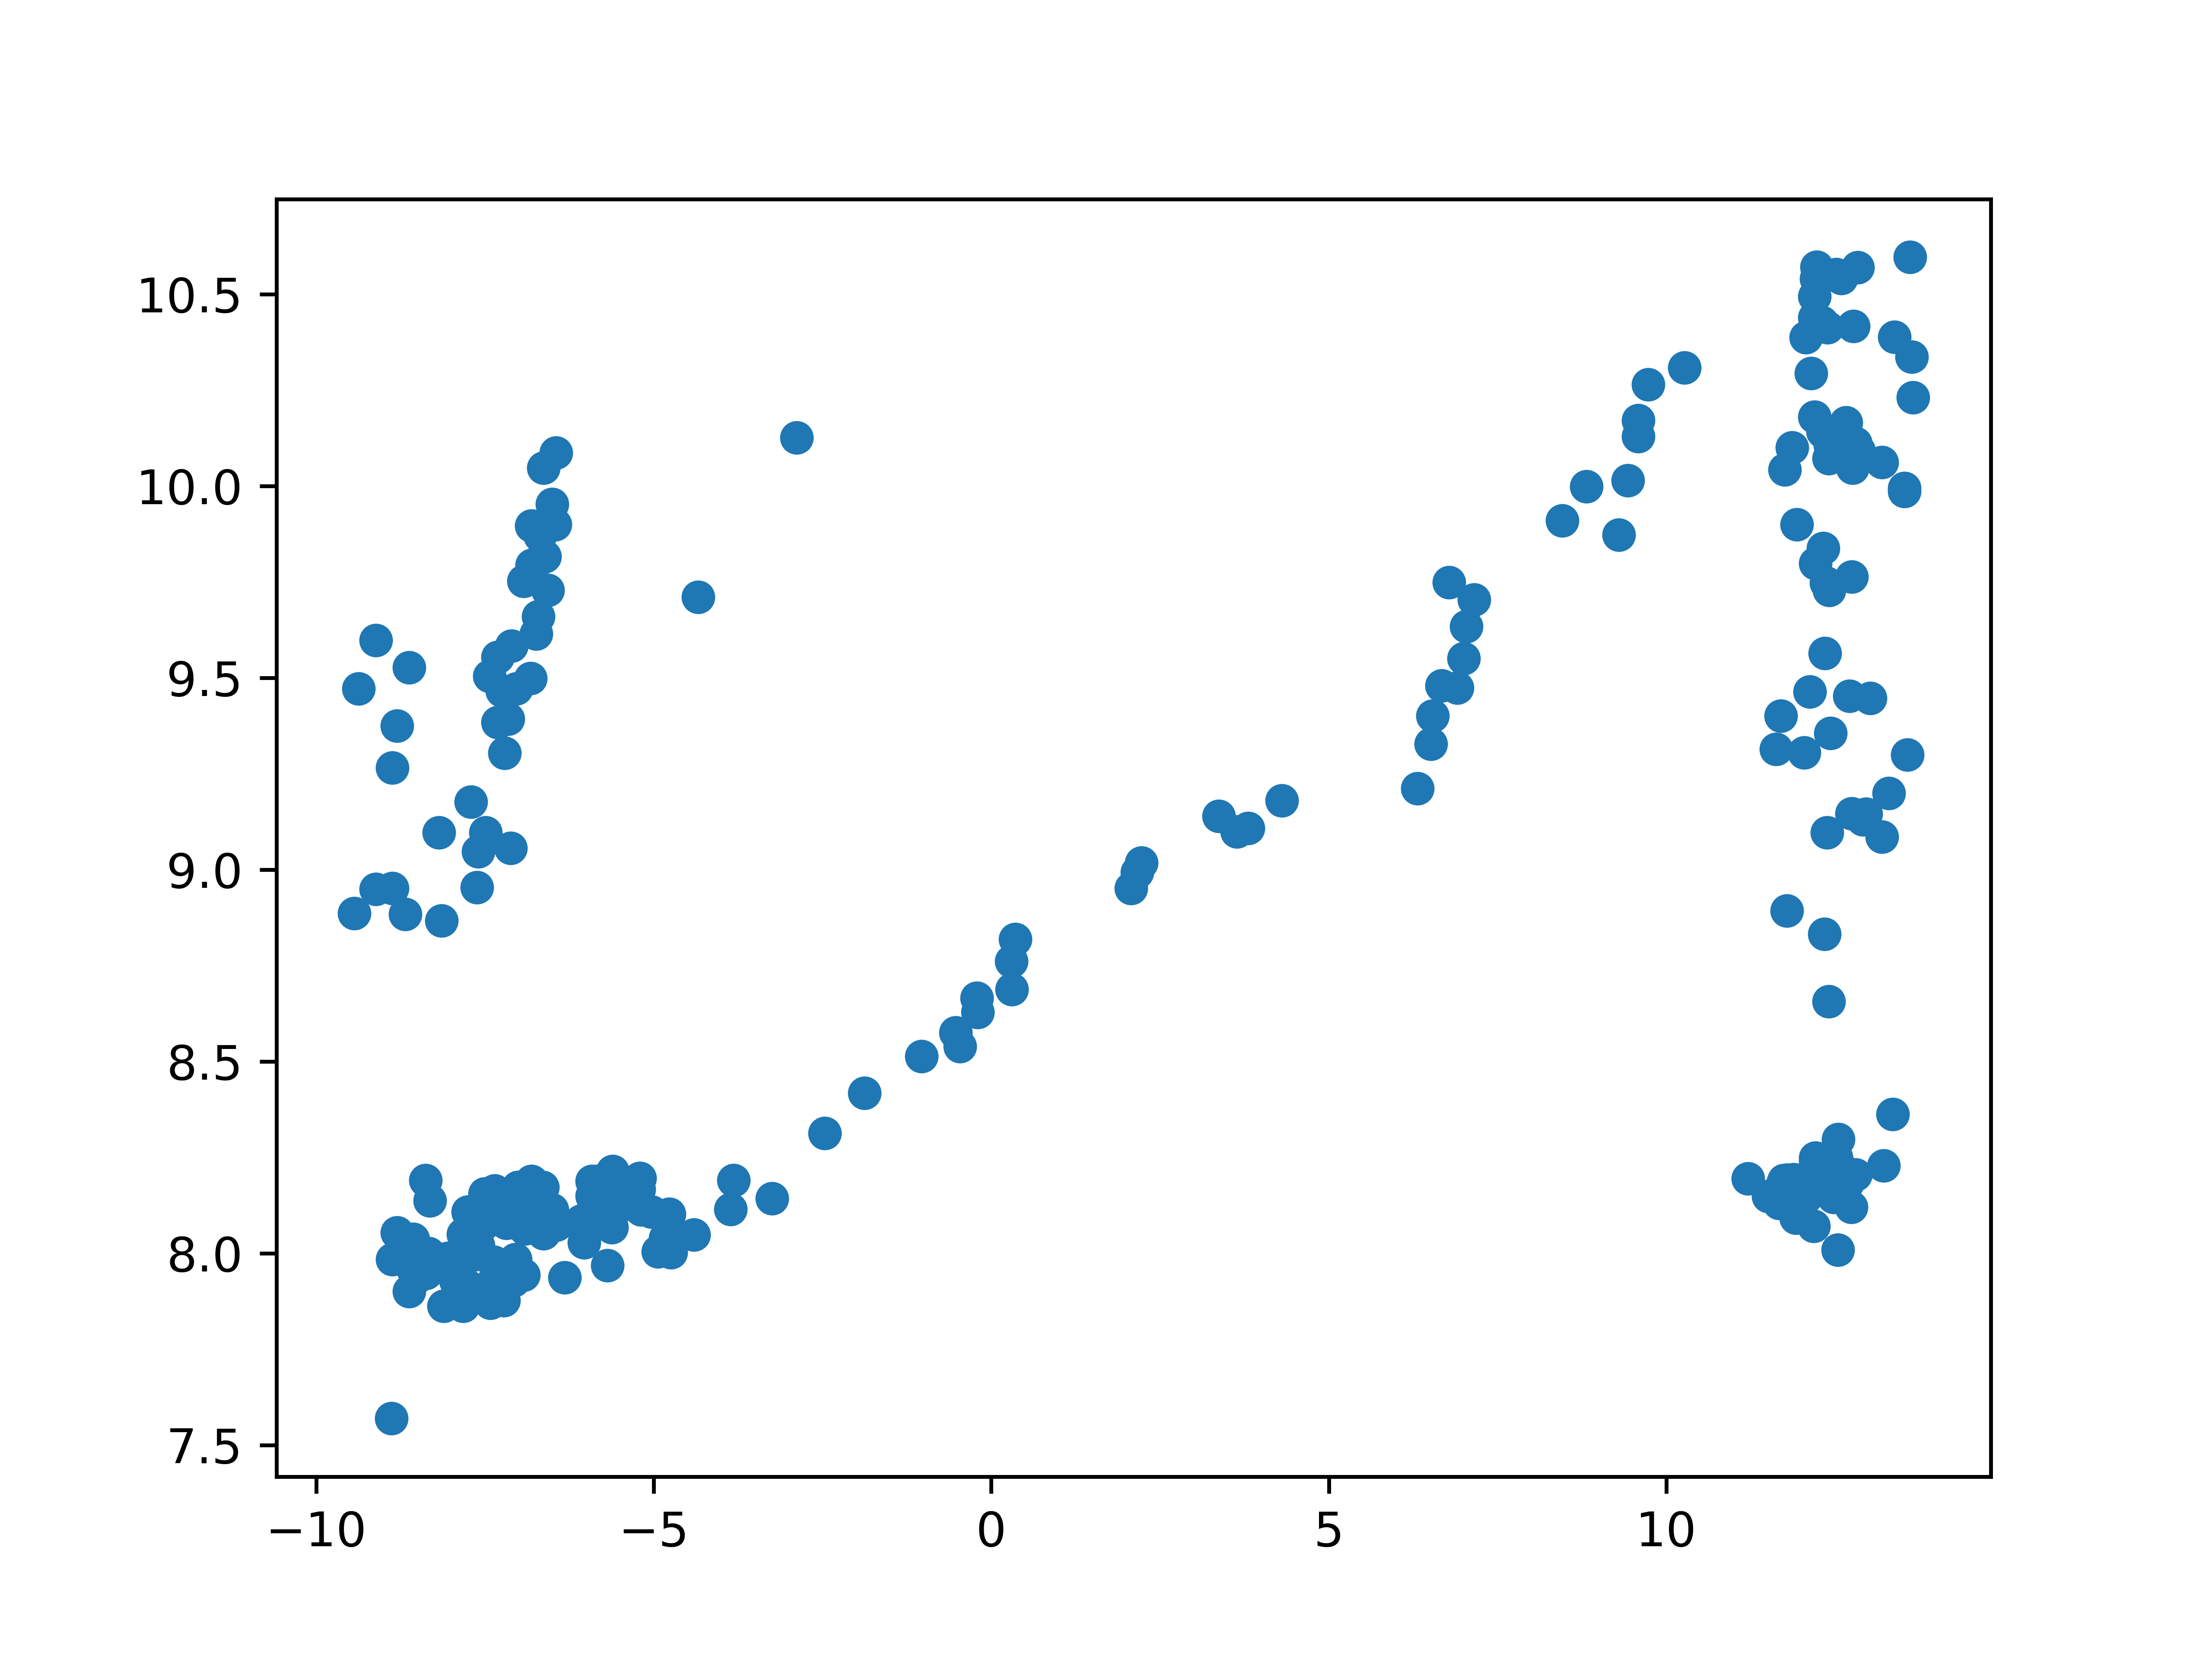
\includegraphics[width = \textwidth]{2Plot2.png}
    \caption{A graph of \(\log{Luminosity}\) vs \(\log{Temperature}\)}
    \label{fig:Fig 2.2}
\end{figure}

\begin{figure}[H]
    \centering
    \includegraphics[width = \textwidth]{2Plot3.png}
    \caption{A graph of \(\log{Luminosity}\) vs \(\log{Temperature}\) for star type 3}
    \label{fig:Fig 2.3}
\end{figure}

\begin{figure}[H]
    \centering
    \includegraphics[width = \textwidth]{2Plot4_2.png}
    \caption{A graph of \(\log{Luminosity}\) vs \(\log{Temperature}\) for star type 3, with degree 2}
    \label{fig:Fig 2.4}
\end{figure}

\begin{figure}[H]
    \centering
    \includegraphics[width = \textwidth]{2Plot4_10.png}
    \caption{A graph of \(\log{Luminosity}\) vs \(\log{Temperature}\) for star type 3, with degree 10}
    \label{fig:Fig 2.5}
\end{figure}

\begin{figure}[H]
    \centering
    \includegraphics[width = \textwidth]{2Plot4_15.png}
    \caption{A graph of \(\log{Luminosity}\) vs \(\log{Temperature}\) for star type 3, with degree 15}
    \label{fig:Fig 2.6}
\end{figure}

\begin{figure}[H]
    \centering
    \includegraphics[width = \textwidth]{2Plot4_16.png}
    \caption{A graph of \(\log{Luminosity}\) vs \(\log{Temperature}\) for star type 3, with degree 16}
    \label{fig:Fig 2.7}
\end{figure}

\begin{figure}[H]
    \centering
    \includegraphics[width = \textwidth]{2Plot4_17.png}
    \caption{A graph of \(\log{Luminosity}\) vs \(\log{Temperature}\) for star type 3, with degree 17}
    \label{fig:Fig 2.8}
\end{figure}

\begin{figure}[H]
    \centering
    \includegraphics[width = \textwidth]{2Plot4_20.png}
    \caption{A graph of \(\log{Luminosity}\) vs \(\log{Temperature}\) for star type 3, with degree 20}
    \label{fig:Fig 2.9}
\end{figure}

\begin{figure}[H]
    \centering
    \includegraphics[width = \textwidth]{2Plot4_25.png}
    \caption{A graph of \(\log{Luminosity}\) vs \(\log{Temperature}\) for star type 3, with degree 25}
    \label{fig:Fig 2.10}
\end{figure}

\begin{figure}[H]
    \centering
    \includegraphics[width = \textwidth]{2Plot4_30.png}
    \caption{A graph of \(\log{Luminosity}\) vs \(\log{Temperature}\) for star type 3, with degree 30}
    \label{fig:Fig 2.11}
\end{figure}

\begin{figure}[H]
    \centering
    \includegraphics[width = \textwidth]{2Plot5.png}
    \caption{A graph of \(\frac{L}{a}\) vs T}
    \label{fig:Fig 2.12}
\end{figure}
Write to

\subsection{Appendix}
\begin{minted}{py}
# Task 2

import numpy as np
import pandas as pd
import matplotlib.pyplot as plt
import operator
from sklearn.preprocessing import PolynomialFeatures as pf
from sklearn.linear_model import LinearRegression
from sklearn.metrics import mean_squared_error
from scipy.optimize import curve_fit
from math import pi

# creating empty list
A_list=[]

# importing the data to be analysed
data = pd.read_csv('Q2a__HR_Diagram.csv')

# grouping the data given by star type
data.groupby(['Star type'])

# setting parameters for plotting
plt.figure(figsize=(7.5, 10.5))
plt.rcParams['font.family'] = 'STIXGeneral'
plt.rcParams['mathtext.fontset'] = 'stix'
plt.rcParams['font.size'] = 12
plt.rcParams['font.weight'] = 'normal'
plt.minorticks_on()
plt.grid(visible=True, which='major', linestyle='-')
plt.grid(visible=True, which='minor', linestyle='--')

# plotting scatter plot for the data given
plt.scatter((data['Temperature/K']), data['Luminosity(L/Lo)'], color='k')
plt.ylabel('L/Lo')
plt.xlabel('T/K')
plt.title('A graph of Luminosity vs Temperature')
plt.savefig('2Plot1.png', dpi=800)
plt.close()

# setting parameters for plotting
plt.figure(figsize=(7.5, 10.5))
plt.rcParams['font.family'] = 'STIXGeneral'
plt.rcParams['mathtext.fontset'] = 'stix'
plt.rcParams['font.size'] = 12
plt.rcParams['font.weight'] = 'normal'
plt.minorticks_on()
plt.grid(visible=True, which='major', linestyle='-')
plt.grid(visible=True, which='minor', linestyle='--')


# plotting log of the data
plt.scatter(np.log(data['Temperature/K']), np.log(data['Luminosity(L/Lo)']), color='k')
plt.ylabel(r'$\log{L/Lo}$')
plt.xlabel(r'$\log{T/K}$')
plt.title(r'A graph of $\log{Luminosity}$ vs $\log{Temperature}$')
plt.savefig('2Plot2.png', dpi=800)
plt.close()

# setting parameters for plotting
plt.figure(figsize=(7.5, 10.5))
plt.rcParams['font.family'] = 'STIXGeneral'
plt.rcParams['mathtext.fontset'] = 'stix'
plt.rcParams['font.size'] = 12
plt.rcParams['font.weight'] = 'normal'
plt.minorticks_on()
plt.grid(visible=True, which='major', linestyle='-')
plt.grid(visible=True, which='minor', linestyle='--')

# dropping the unwanted values
value_3 = data.mask(data['Star type']!=3).dropna().reset_index()
plt.scatter(np.log(value_3['Temperature/K']), np.log(value_3['Luminosity(L/Lo)']), color='k')
plt.ylabel(r'$\log{L/Lo}$')
plt.xlabel(r'$\log{T/K}$')
plt.title(r'A graph of $\log{\mathrm{Luminosity}}$ vs $\log{\mathrm{Temperature}}$ for star type 3')
plt.savefig('2Plot3.png', dpi=800)
plt.close()

# listing a number of the tried degree values
degrees = np.array([2, 10, 20, 30, 25, 15, 16, 17])
# creating a loop to test each degree until the smallest rmse is obtained and plotting each test

for i in degrees:
    # obtaining the log of the wanted data
    y = np.log(value_3['Luminosity(L/Lo)'])
    x = np.log(value_3['Temperature/K'])

    # reshaping the array
    x_a = x.array.reshape(-1,1)  # type: ignore
    poly = pf(degree=i)
    poly_Lumen=poly.fit_transform(x_a)

    model = LinearRegression()
    model.fit(poly_Lumen, y)
    y_pred = model.predict(poly_Lumen)

    rmse = np.sqrt(mean_squared_error(y, y_pred))
    print(f'The root mean square is: {rmse}, with the degree of freedom is: {i}')

    plt.figure(figsize=(7.5, 10.5))
    plt.rcParams['font.family'] = 'STIXGeneral'
    plt.rcParams['mathtext.fontset'] = 'stix'
    plt.rcParams['font.size'] = 12
    plt.rcParams['font.weight'] = 'normal'
    plt.minorticks_on()
    plt.grid(visible=True, which='major', linestyle='-')
    plt.grid(visible=True, which='minor', linestyle='--')

    plt.scatter(x, y, color='k')
    sort_axis = operator.itemgetter(0)
    sorted_zip = sorted(zip(x, y_pred), key=sort_axis)
    x, y_pred = zip(*sorted_zip)
    plt.plot(x, y_pred, color='k')
    plt.xlabel(r'$\log{T/K}$')
    plt.ylabel(r' Predicted Luminosity')
    plt.title(f'A graph of Temperature vs Luminosity with degree {i}')
    #plt.savefig(f'2Plot4_{i}.png', dpi=800)
    plt.close()

# importing the filtered data to be analysed
data2 = pd.read_csv('Q2b__stars.csv')

# defining each variable
T = data2['Temperature/K']
L = (data2['Luminosity(L/Lo)'])*(3.846e26)
R = data2['Radius(R/Ro)']

# creating a loop to obtain A
for i in range(len(R)):
    a = 4* pi *((R[i]*6.957e8)**2)
    A_list.append(a)

A = np.array(A_list)

# calculating the L/A
L_A = L/A

# defining a function to fit to
def fit_func(T, sigma):
    return sigma * (np.power(T, 4))

# creating a linspace to obtain a smoother curve
T_lin = np.linspace(T.min(), T.max(), 1000)

# using curve fit to obtain the best fitting curve
popt, pcov = curve_fit(fit_func, T, L_A)
fit_line = fit_func(T_lin, popt[0])

# plotting the graph
f = plt.figure(figsize=(7.5, 10.5))
plt.rcParams['font.family'] = 'STIXGeneral'
plt.rcParams['mathtext.fontset'] = 'stix'
plt.rcParams['font.size'] = 12
plt.rcParams['font.weight'] = 'normal'
plt.title(r'A graph of $\frac{\mathrm{L}}{\mathrm{A}}$ against T')
plt.scatter(T, L_A, color='k')
plt.plot(T_lin, fit_line, color='k')
plt.minorticks_on()
plt.grid(visible=True, which='major', linestyle='-')
plt.grid(visible=True, which='minor', linestyle='--')
plt.xlabel(r'T/K')
plt.ylabel(r'$\frac{\mathrm{L}}{\mathrm{A}}$ /Wm$^{-2}$')
plt.savefig('2Plot5.png', dpi=800)

# theoretical boltzmann constant
sigma_theoretical = 5.6696e-8 

boltz_accu = ((popt[0]/sigma_theoretical)-1)*100

# displaying the boltzamnn constant
print(f'The Boltzmann constant is: {popt[0]:.2E}, with a precision of {boltz_accu}')

# importing the third set of data
table_2_data = pd.read_excel('Q2c__Table_2_Data.xlsx')

L_data = (table_2_data['L/L0'])*(3.846e26)    
T_data = table_2_data['T/K']                              

# calculating the theoretical radii
r_theoretical = np.sqrt((L_data)/((4)*(pi)*(sigma_theoretical)*(T_data**4)))
print(f'Theoretical stellar radius: {r_theoretical}')

# calculating the experimental radii
r_experimental = np.sqrt((L_data)/((4)*(pi)*(popt[0])*(T_data**4)))
print(f'Experimental stellar radius: {r_experimental}')

for i in range(len(r_experimental)):
    r_accuracy = abs((r_experimental[i]/r_theoretical[i])-1)*100
    print(r_accuracy)

\end{minted}

\section{Task 3 - Exponential Curve Fitting}

\subsection{Introduction and Theoretical Background}
In certain cases an exponential fit is required in order to fit the trendline to the data given, one such example was tackled in this task. It was required to obtain a trendline to the exponential decay of radioactive substances. However, this highlights the fact that the initial guesses that are given to the function must be ideal in order to obtain the ideal trendline.

\subsection{Materials and Methods}
\subsubsection{Languages and Packages}
Python 3.10.8, Pandas, Numpy, Mathplotlib.pyplot, Seaborn, Scipy, Sklearn. 

\subsubsection{Methodology}
\begin{enumerate}
    \item The data for Calcium was selected, this was when the atomic number, Z was equal to 20. The exponential regression line was fitted to this data and the half-life was obtained.
    \item The same procedure was repeated for all the unstable isotopes in the dataset. 
    \item A list for the proton number, neutron number and half-lives was created and this was plotted using the seaborn heatmap function. A straight line was plotted accordingly to show the valley of stability by plotting a line for when Z=N.
\end{enumerate}

\subsection{Results}
\begin{table}[H]
    \centering
    \begin{tabular}{|c|c|}
    \hline
    t\(_{\frac{1}{2}\mathrm{ exponential}}\)/\(\times 10^{-8}\)s & 3.54 \\ \hline
    t\(_{\frac{1}{2}\mathrm{ lineral}}\)/\(\times 10^{-8}\)s & 3.54 \\ \hline
    \end{tabular}
    \caption{Table of Calcium Half-life}
    \label{tab: Table 3.1}
\end{table}

\subsection{Discussion}
In this task it was required to find the half life of many istopes of different elements. One of the cases was for calclium-14. This was don by first selecting the data for when Z=20 and applying a \mintinline{py}{curve_fit} on the data using the following equation:
\begin{equation}
    \frac{A}{A_0} = \exp\left(-\frac{t\ln2}{t_\frac{1}{2}}\right) ,
\end{equation}
the resultant fit can be seen in the top half of figure
~\ref{fig:Fig 3.2}. In addition to this the straight line fit of the data was plotted in order to compare both ways to find the half-life. In the case of the logarithmic case the equation then becomes:
\begin{equation}
    \log{A} = A_0-\frac{\ln2}{t_{\frac{1}{2}}}t ,
\end{equation}
the result of this linear equation can be seen in the lower part of the figure \ref{fig:Fig 3.2}. One can see from the results show in the table \ref{tab: Table 3.1} that both methods result in the same value for the half-life. The \mintinline{py}{curve_fit} method was then used on all of the data given, which resulted in a list of half-lives. This list was then appened with the corresponding Z number and N number in order to obtain the final table of all values to be used for later plotting. These results were then passed thorugh the code in order to obtain the heat map that can be seen in figure \ref{fig:Fig 3.3}. One should note that the central white dots are the stable isotopes in the valley of stability \parencite{macintosh2001m} and that the black straight line going through the plot is the line of Z=N. It should also be noted that the valley of stability does not follow a proportional increase after Z=20 \parencite{boutin2002climbing}. This is as isotopes with more than 20 protons require more than 20 neutrons in order to be stable \parencite{macintosh2001m}.

\subsection{Figures and Graphs}
\begin{figure}[H]
    \centering
    \includegraphics[width = \textwidth]{3Plot1.png}
    \caption{A graph of \(\log{A}\) vs \(\log{T}\)}
    \label{fig:Fig 3.1}
\end{figure}

\begin{figure}[H]
    \centering
    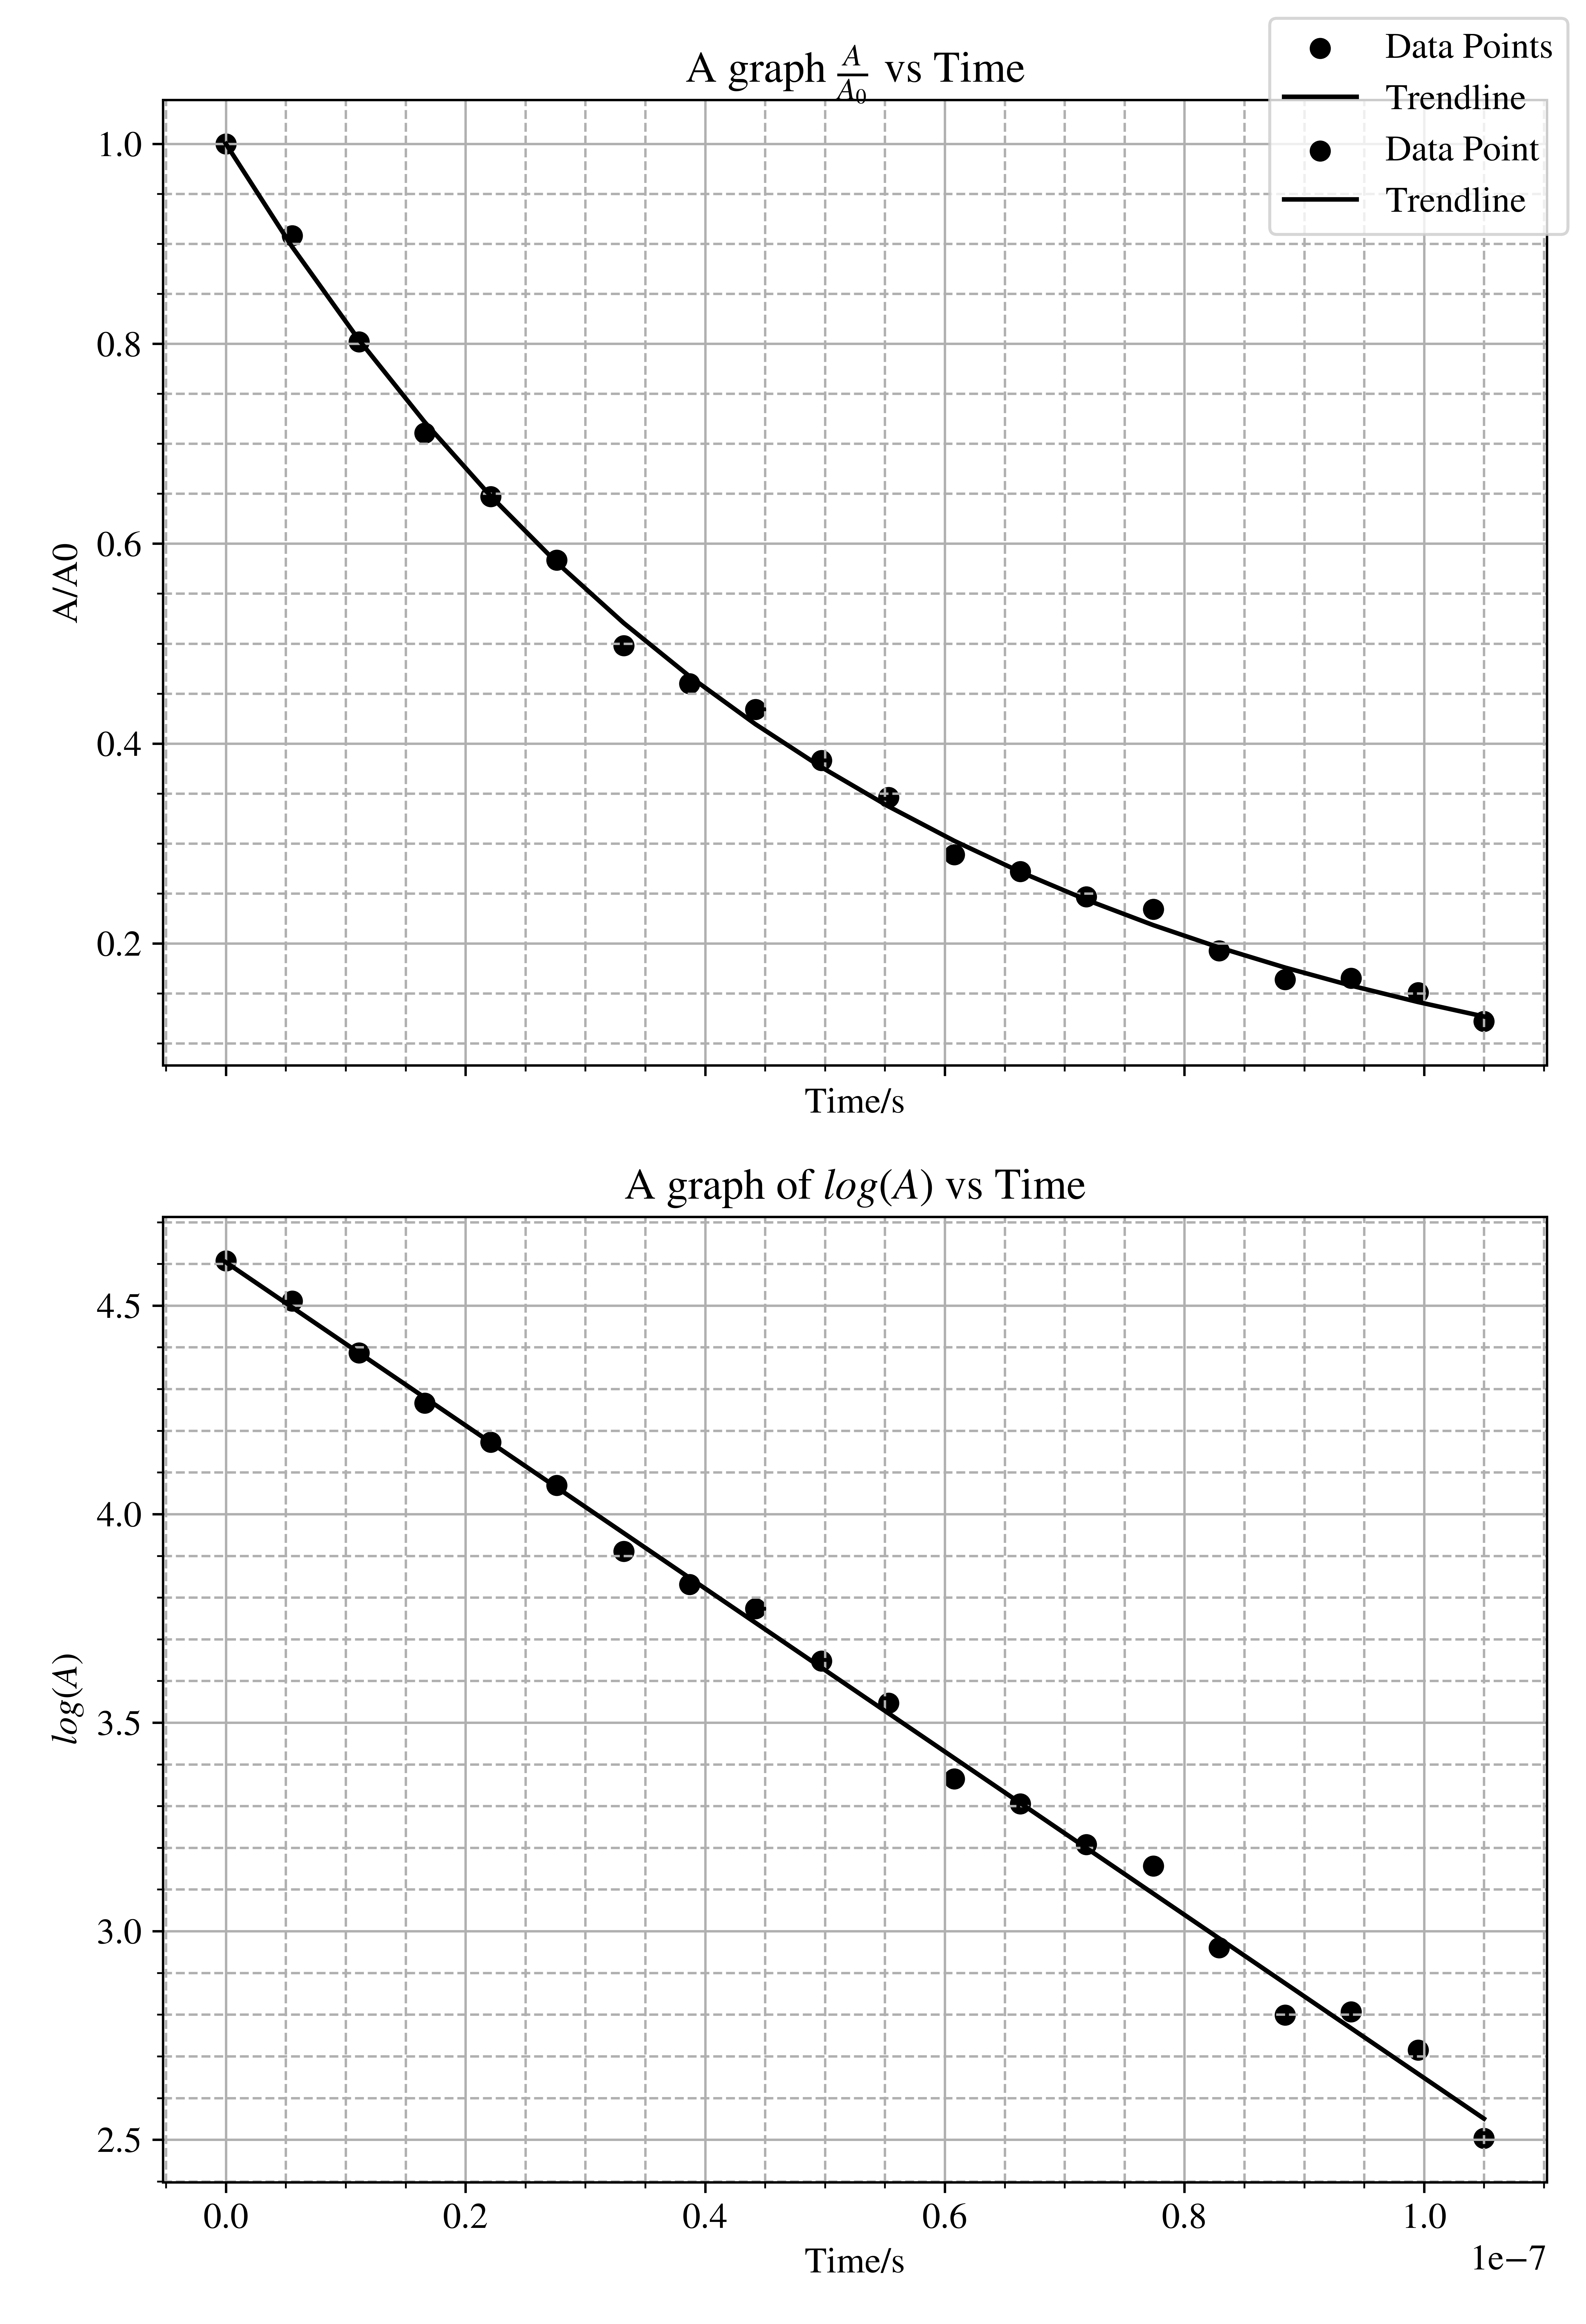
\includegraphics[width = \textwidth]{3Plot2.png}
    \caption{A graph of \(\frac{A}{A_0}\) vs T and subplot of \(\log{A}\) vs \(\log{T}\)}
    \label{fig:Fig 3.2}
\end{figure}

\begin{figure}[H]
    \centering
    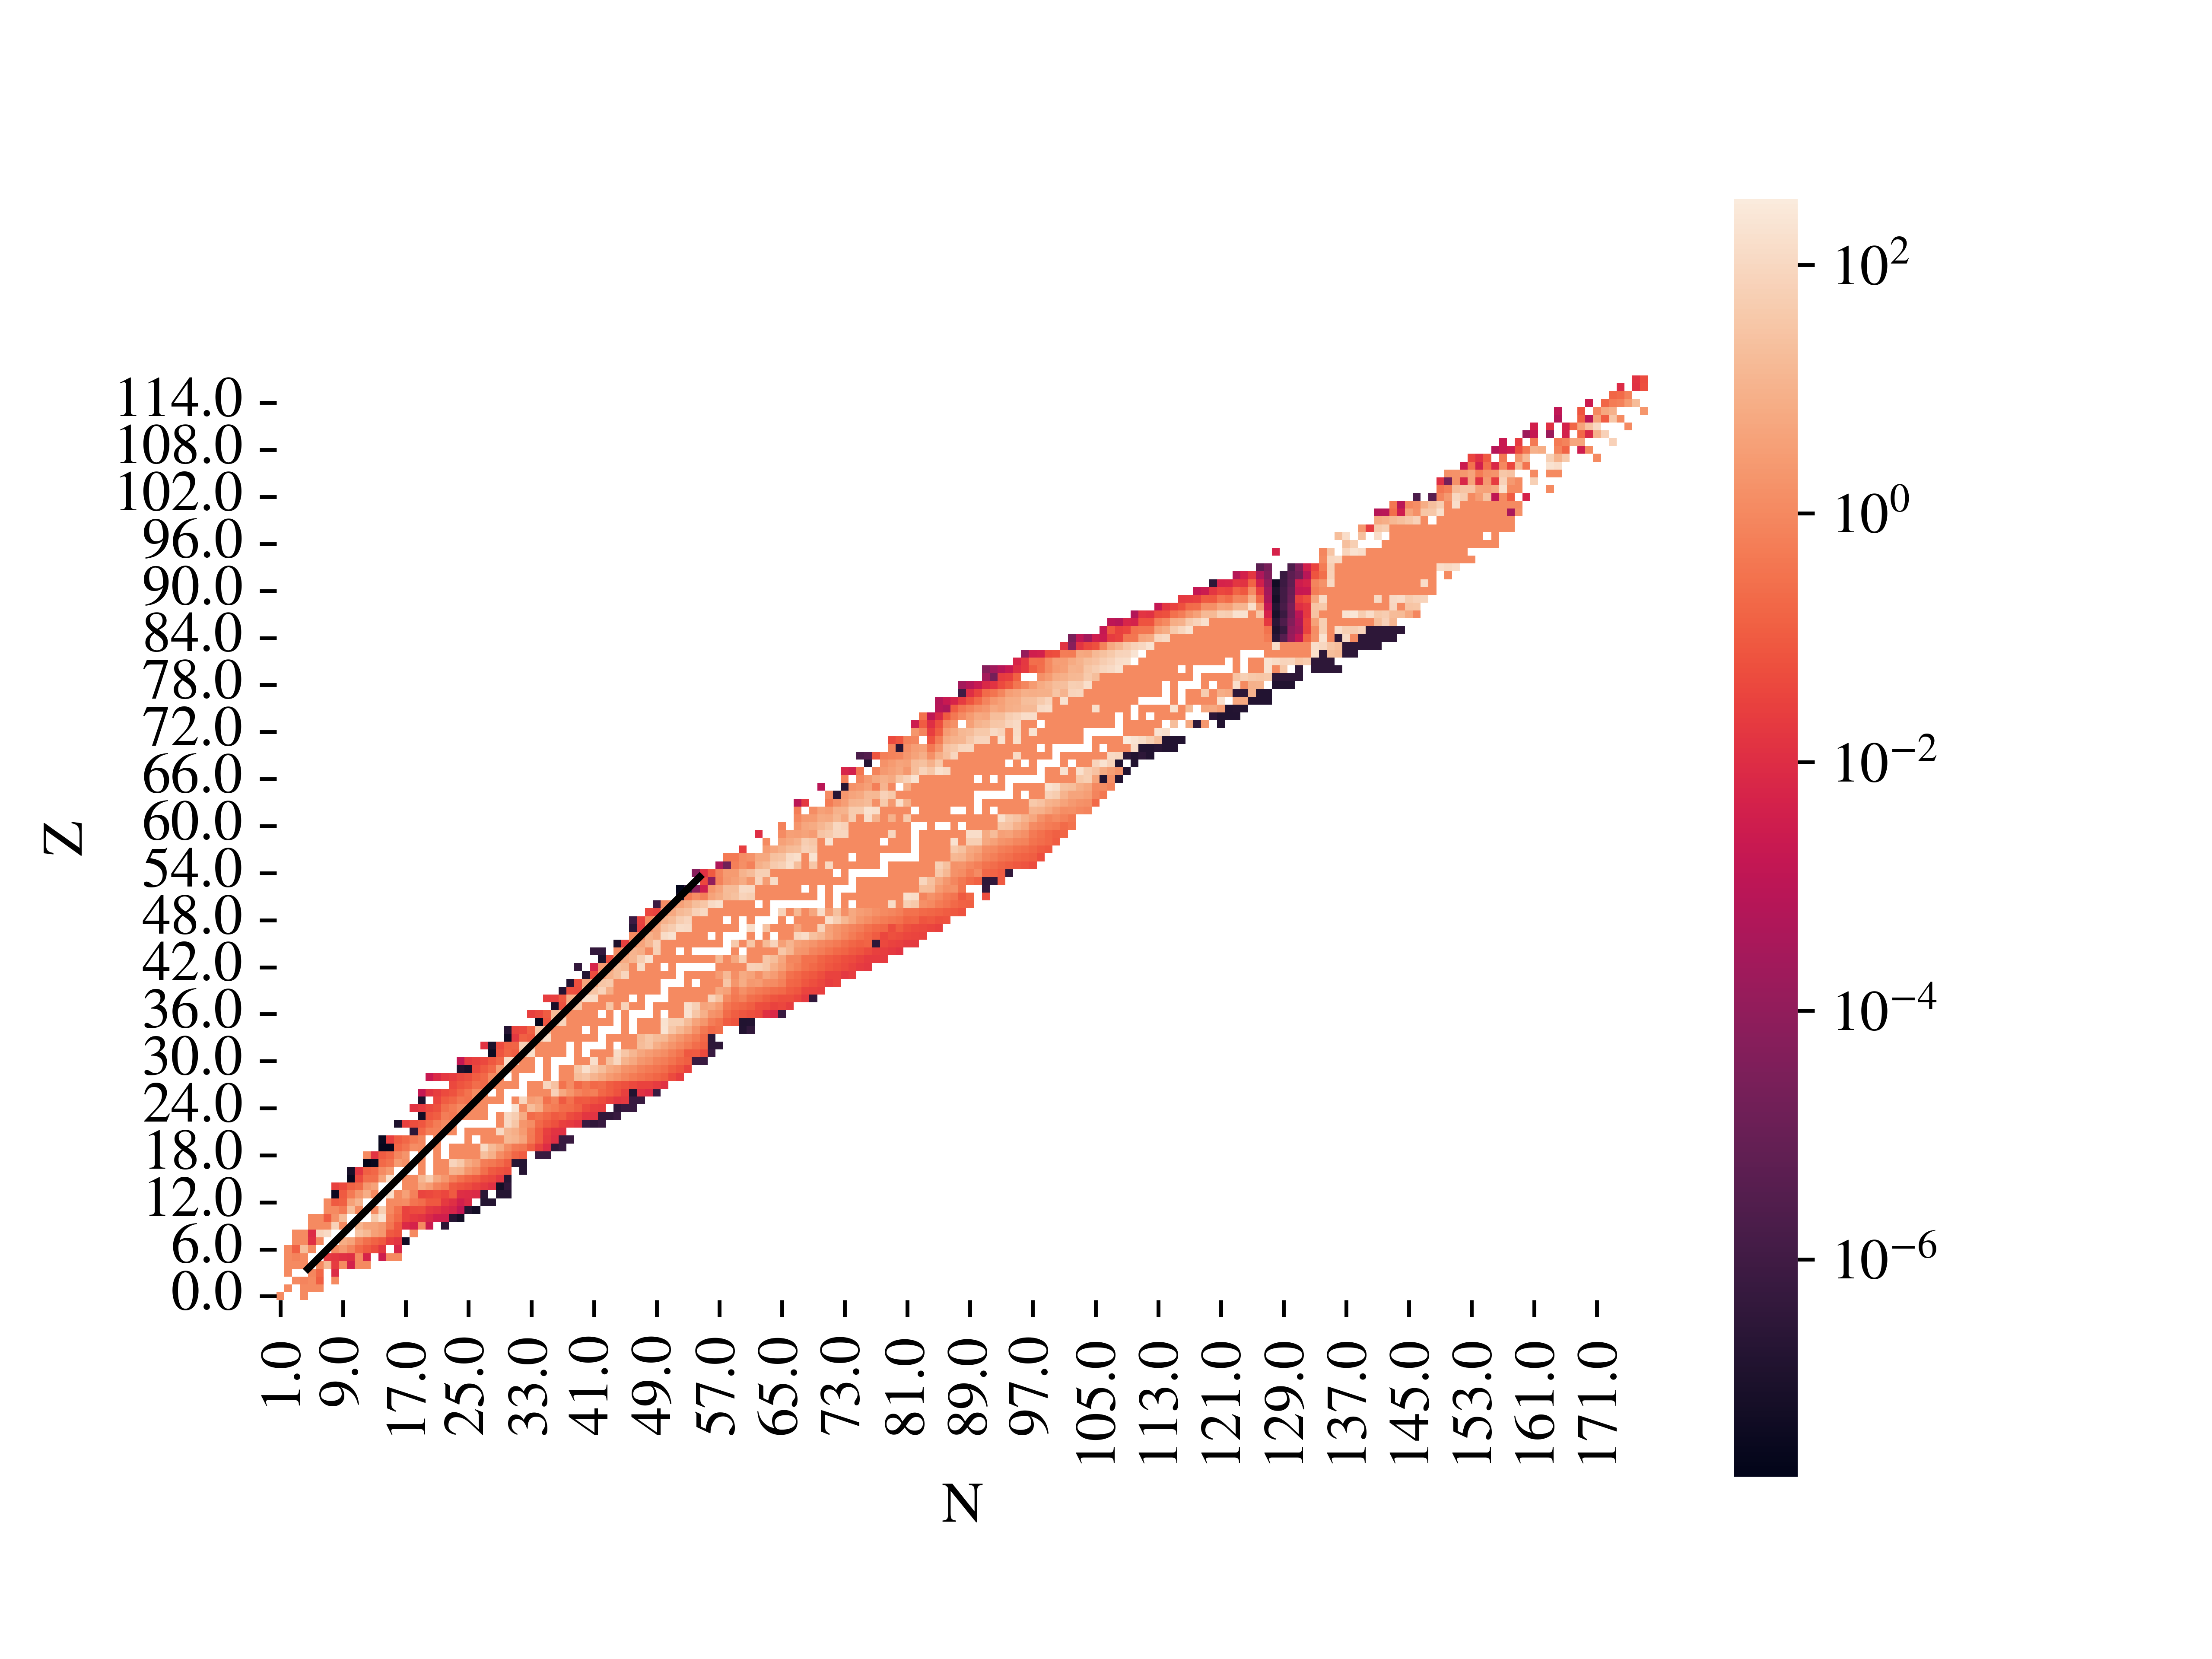
\includegraphics[width = \textwidth]{3Plot3.png}
    \caption{A heat map of the Z vs N with the stability line}
    \label{fig:Fig 3.3}
\end{figure}

\subsection{Appendix}
\begin{minted}{py}
# Task 3

from matplotlib.colors import LogNorm
import numpy as np
import pandas as pd
import matplotlib.pyplot as plt
import seaborn as sns
from sklearn.metrics import mean_squared_error
from scipy.optimize import curve_fit

# importing the data to be analysed
data = pd.read_csv('Q3__Isotope_Decay_Dataset.csv')

# initialising the lists to be used
index_list=[]
slice_list=[]
lst = []
half_life_list = []
z_list = []
n_list = []
new_list =[]
new_z_list = []
new_n_list = []

# defining array to be used
even_a = np.arange(0,5922,2)
odd_a = np.arange(1,5921,2)

# importing specific data for A
a_values = data['A']
# creating an index with the data selected
index_array = np.arange(0, len(a_values)+20, 20)

# finding the ean values of A for each isotope, 20 values each
mean_a = [np.mean(a_values.iloc[index_array[i]:index_array[i+1]]) for i in range(len(index_array)-1)]

# finding which values of the mean are lower than 95 to account for the noise of the values and storing their index
for i in range(len(mean_a)):
    if mean_a[i] < 95:
        index_list.append(i)

# creating new list to slice the data according to the indices from before
for i in range(len(index_list)):
    slice_list.append((index_list[i])*20)
    slice_list.append((index_list[i]+1)*20)

# keeping only the data for the unstable isotopes
data_sliced = [data.iloc[slice_list[even_a[i]]:slice_list[odd_a[i]]] for i in range(len(even_a)-1)]

# removing any empty values
data_sliced = list(filter(lambda df: not df.empty, data_sliced))

# defining an empty dataframe
df = pd.DataFrame(columns=['z','n','t/s','A'])

# creating a dataframe with the sliced values for later use
for i in range(len(data_sliced)):
    temp_df = pd.DataFrame(data_sliced[i], columns=['z', 'n', 't/s', 'A'])
    df = pd.concat([df,temp_df]).reset_index(drop=True)

# indexing the new dataframe
index_df = np.arange(0, len(df), 1)
df.reset_index(drop=True).set_index(index_df, inplace=True)

# selecting only the data for A and t
a_uvalues = df['A']
t_values = df['t/s']

# finding the mean for A and t for each isotope
mean_ua = [np.mean(a_uvalues.iloc[index_array[i]:index_array[i+1]]) for i in range(len(index_array)-1)]
mean_t = [np.mean(t_values.iloc[index_array[i]:index_array[i+1]]) for i in range(len(index_array)-1)]

# edfinign the plotting parameters
plt.figure(figsize=(7.5, 10.5))
plt.rcParams['font.family'] = 'STIXGeneral'
plt.rcParams['mathtext.fontset'] = 'stix'
plt.rcParams['font.size'] = 12
plt.rcParams['font.weight'] = 'normal'
plt.minorticks_on()
plt.grid(visible=True, which='major', linestyle='-')
plt.grid(visible=True, which='minor', linestyle='--')
plt.tight_layout()

# plotting the data
plt.scatter(np.log(mean_t), np.log(mean_ua), color='k')
plt.savefig('3Plot1.png', dpi=800)
plt.close()

# selecting the data only for calcium
calcium_df = df[df['z']==20]
# selecting only the data for 1 calcium isotope
calcium_df = df.iloc[5680:6080]
# re-indexing
calcium_df.reset_index(drop=True, inplace=True)

# defining the values and data to be used for calcium
calcium_a = calcium_df['A'][0:20]
calcium_log_a = np.log(calcium_df['A'][0:20])
calcium_t = (calcium_df['t/s'][0:20])

# defining the function to find the value of A/A0
def fit_func(t, thalf):
    return (np.exp((-1 * t * np.log(2))/thalf))

# using curve fit to calculate the value of the half life
popt, pcov = curve_fit(fit_func, calcium_t, (calcium_a/calcium_a[0]))

# obtaining the curve of the calclium isotope decay
fitted_line = fit_func(calcium_t, popt[0])
print(f'The half life of calcium-14 is: {popt[0]:.2E}s')

# obtaining the straight line to compare values obtained
coeffs, cov = np.polyfit(calcium_t, calcium_log_a, 1, cov=True)
polyfunc = np.poly1d(coeffs)
trendline = polyfunc(calcium_t)

print(f'The half life of calcium-14 is from the srtaight line graph: {-np.log(2)/coeffs[0]:.2E}s')

# defining the subplots
f, (a0, a1) = plt.subplots(2, 1, sharex=True, sharey=False, figsize=(7.3, 10.7))

# defining the font to be used
plt.rcParams['font.family'] = 'STIXGeneral'
plt.rcParams['mathtext.fontset'] = 'stix'
plt.rcParams['font.size'] = 12
plt.rcParams['font.weight'] = 'normal'

# plotting the curve
a0.scatter(calcium_t, (calcium_a/calcium_a[0]), color='k', label='Data Points')
a0.plot(calcium_t, fitted_line, color='k', label='Trendline')
a0.minorticks_on()
a0.grid(visible=True, which='major', linestyle='-')
a0.grid(visible=True, which='minor', linestyle='--')
a0.set_xlabel('Time/s')
a0.set_ylabel('A/A0')
a0.set_title(r'A graph $\frac{A}{A_0}$ vs Time')

# plotting the straight line
a1.scatter(calcium_t, calcium_log_a, color='k', label='Data Point')
a1.plot(calcium_t, trendline, color='k', label='Trendline')
a1.minorticks_on()
a1.grid(visible=True, which='major', linestyle='-')
a1.grid(visible=True, which='minor', linestyle='--')
a1.set_xlabel('Time/s')
a1.set_ylabel(r'$log(A)$')
a1.set_title(r'A graph of $log(A)$ vs Time')

# removing the excess space, showing legend and saving figure
f.tight_layout()
f.legend()
f.savefig('3Plot2.png', dpi=800)
plt.close()

# defining specific data columns
df_t = df['t/s']
df_a = df['A']

# creating array for selections of data
selection_array = np.arange(0, len(df['t/s']), 20)

# applying the curve fit function on all of the data
for i in range(len(selection_array)-1):
    da = df_a[selection_array[i]:selection_array[i+1]]
    dt = df_t[selection_array[i]:selection_array[i+1]]
    da0 = df_a[selection_array[i]]
    da_da0 = da/da0
    popt, pcov = curve_fit(fit_func, dt, da_da0)
    half_life_list.append(popt[0])
    z_list.append(df['z'][selection_array[i]])
    n_list.append(df['n'][selection_array[i]])

# joining the 3 lists together
plotting_data = list(zip(z_list, n_list, half_life_list))

# creating a data frame for Z, N, Half life
results_df = pd.DataFrame({'Z':z_list, 'N': n_list, 'Half Life/s': half_life_list})
results_df.to_excel('Table.xlsx')
plot_data = results_df.pivot(index='Z', columns='N',
values='Half Life/s')

# defining the font to be used
plt.rcParams['font.family'] = 'STIXGeneral'
plt.rcParams['mathtext.fontset'] = 'stix'
plt.rcParams['font.size'] = 12
plt.rcParams['font.weight'] = 'normal'

# plotting the Heat map
ax = sns.heatmap(plot_data, square=True, norm=LogNorm())
ax.invert_yaxis()

# finding the index for when Z = N
for i in range(len(results_df)):
    if results_df['Z'][i] == results_df['N'][i]:
        new_list.append(i)

# selecting the data for when Z = N
for i in new_list:
    new_z_list.append(z_list[i])
    new_n_list.append(n_list[i])

# changing the data from before of Z = N, into a dataframe
z_n = pd.DataFrame({'Z': new_z_list, 'N': new_n_list}) 

# plotting the straight line for the data
plt.plot(z_n['N'], z_n['Z'], color='k')

# saving the figure
plt.savefig('3Plot3.png', dpi=800)

\end{minted}

\section{Task 4 - Periodic Curve Fitting}

\subsection{Introduction and Theoretical Background}
In some cases neither of the linear, curve or exponential regression would fit the trendline according to the data, as the data would have a clear periodic property. One of such cases is the data of the orbit of moons around a planet. In this case the orbital data for the 4 innermost moons of Jupiter was considered. 

As this task deals with orbital data, one should consider the 3 Kepler Laws. Kepler's first law states that \textit{``the orbit of a planet is elliptical and that the Sun is positioned at one focus''} \parencite{muncaster}. The second law states that \textit{``a line joining the planet to the Sun sweeps out equal areas in equal time
intervals''} \parencite{muncaster}. Furthermore, the third law states that \textit{``the orbital period of a planet squared is proportional to the semi-major axis
cubed''} \parencite{muncaster}. Additionally, one must consider that if a moon with mass \textit{m} is orbiting a planet with mass \textit{M}, the centripital force is equal to the gravitational force \parencite{muncaster}. If one uses this consideration in conjuction with Kepler's third law the following equation is obtained:
\begin{equation}
    T^2 = \frac{4\pi^2r^3}{\mathrm{GM}}
    \label{eq: equation 4.1}
\end{equation}

\subsection{Materials and Methods}
\subsubsection{Languages and Packages}
Python 3.10.8, Pandas, Numpy, Matplotlib.pyplot, Scipy.

\subsubsection{Methodology}
\begin{enumerate}
    \item The data for the first moon Io was first plotted in order to get an idea of how the position moves periodically about the 0 point. From this behaviour it was noted that the parameters to be used should be the maximum amplitude and the wavelength.
    \item The function taking the two parameters was used for all the moon data in order to obtain all the periodic times and semi-major axis. These values were converted from jupiter diameters and julian data into meteres and seconds respectively.
    \item The previous values were then used to obtain the mass of jupiter by linear regression of equation~\ref{eq: equation 4.1}. 
    \item These values were then used in conjuction with the gravitaional foces of jupiter on each moon to determine the mass of each moon.
\end{enumerate}

\subsection{Results}
\begin{table}[H]
    \centering
    \begin{tabular}{|c|c|c|c|c|}
    \hline
    Moon Name & Semi Major axis/m & T/s & m/kg & m\(_{accuracy}\) \\ \hline
    Io & 4.2\(\times10^8\) & 151200.02 & 8.71\(\times10^{22}\) & 2.50\% \\ \hline
    Europa & 6.6\(\times10^8\) & 307583.91 & 4.81\(\times10^{22}\) & 0.26\% \\ \hline
    Ganymede & 1.1\(\times10^9\) & 617760.01 & 1.44\(\times10^{23}\) & 2.99\% \\ \hline
    Callisto & 1.9\(\times10^9\) & 1425599.87 & 1.06\(\times10^{23}\) & 1.39\% \\ \hline
    \end{tabular}
    \caption{Table of Jupiter's Moon Information}
    \label{tab: Table 4.1}
\end{table}

\begin{table}[H]
    \centering
    \begin{tabular}{|c|c|}
    \hline
    M\(_{jupiter}\) & 1.92\(\times10^{27}\) \textpm 6.77\(\times10^{24}\)kg \\ \hline
    M\(_{percision}\) & 1.12\% \\ \hline
    \end{tabular}
    \caption{Table of Jupiter Information}
    \label{tab: Table 4.2}
\end{table}

\begin{table}[H]
    \centering
    \begin{tabular}{|c|c|}
    \hline
    F\(_{g io}\) & 6.35 \(\times 10^{22}\) \\ \hline
    F\(_{g europa}\) & 1.40 \(\times 10^{22}\) \\ \hline
    F\(_{g ganymede}\) & 1.63 \(\times 10^{22}\) \\ \hline
    F\(_{g callisto}\) & 3.87 \(\times 10^{21}\) \\ \hline
    \end{tabular}
    \caption{Table of Garivational forces on the moons}
    \label{tab: Table 4.3}
\end{table}

\subsection{Discussion}
In order to obtain the periodic time of the orbit of each moon, the \mintinline{py}{curve_fit} was given two paraments. The first parament was the amplitude of each orbit which was simply done by finding the maximum value of each moon positional data, the second parameter was the wavelength or time to reach the same place in the orbit, this was done with a bit of trial and imporvement. The semi-major axis of each planet was then converted to meters by simply multiplying each value by the diameter of jupiter and the conversion from julian date to seconds was simply done by multiplying by \(86400\). The mass of jupiter was then found by inputting the relevant values into equation \ref{eq: equation 4.1} and treating the \(\frac{4\pi^2}{GM}\) as the gradient for the straight line that can be seen in figure \ref{fig:Fig 4.2}. The mass was then found by simply making M the subject of the formula in the aformentioned equation when it was equal to the gradient. The actual mass of jupiter and the actual mass of each of the moon were used with the actual radius in order to calculcate the gravitational force of jupiter on the moon using the following equation:
\begin{equation}
    F_g = \frac{GM_J~m_{moon}}{r^2} .
\end{equation}
The graviatiational forces were then used in conjuction with the experimental value of the mass of jupiter and the radius of the orbit in order to calculate the individual masses of the moon \parencite{muncaster}. 

\subsection{Figures and Graphs}
\begin{figure}[H]
    \centering
    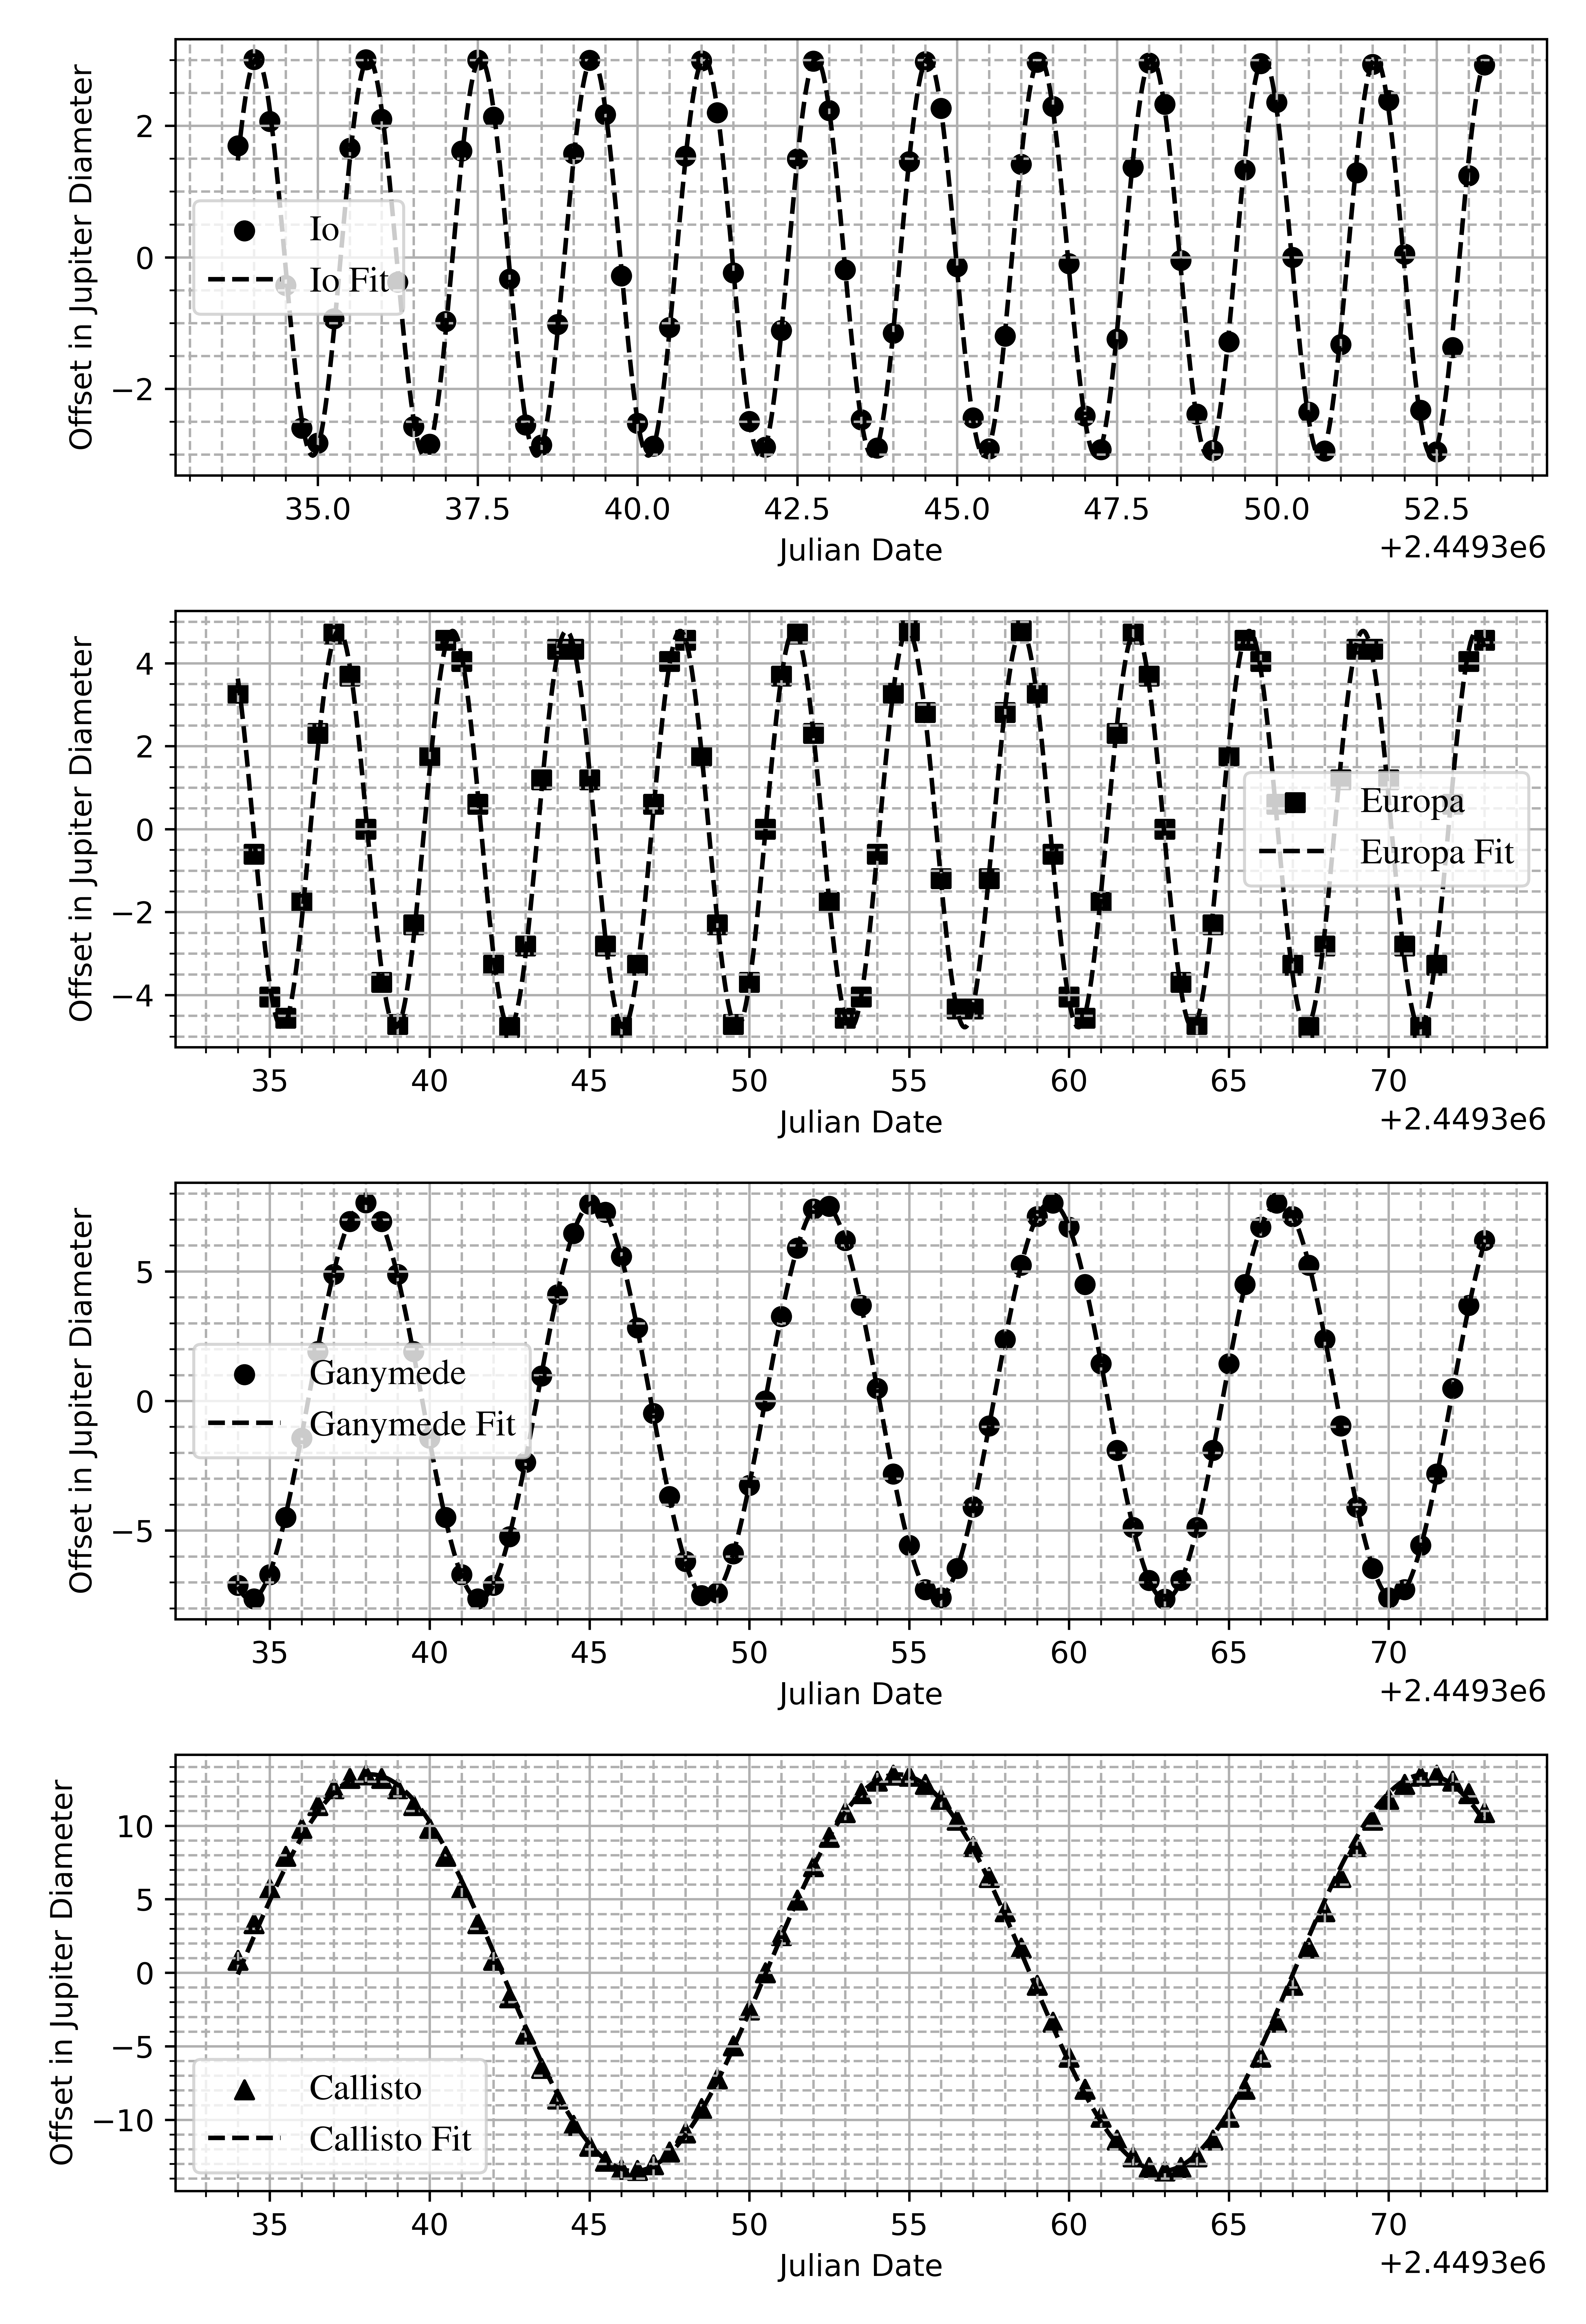
\includegraphics[width = \textwidth]{4Plot1.png}
    \caption{A graph of all moon offset vs julian date waves}
    \label{fig:Fig 4.1}
\end{figure}

\begin{figure}[H]
    \centering
    \includegraphics[width = \textwidth]{4Plot2.png}
    \caption{A graph of \(r^3\) vs \(T^2\)}
    \label{fig:Fig 4.2}
\end{figure}

\newpage

\subsection{Appendix}
\begin{minted}{py}
# Task 4

import pandas as pd
import numpy as np
import matplotlib.pyplot as plt
from scipy.optimize import curve_fit

# importing the data 
data = pd.read_csv('Q4__Galilean_Moon_Astrometric_Data.csv')

# importing the offset data for each moon
io_position = data['Io_Offset (Jup Diameters)']
europa_position = data['Europa_Offset (Jup Diameters)']
ganymede_position = data['Ganymede_Offset (Jup Diameters)']
callisto_position = data['Callisto_Offset (Jup Diameters)']

# importing the hjd data for each moon
io_hjd = data['Io_Julian_Date (HJD)']
europa_hjd = data['Europa_Julian_Date (HJD)']
ganymede_hjd = data['Ganymede_Julian_Date (HJD)']
callisto_hjd = data['Callisto_Julian_Date (HJD)']

# creating linspaces for each moon to obtain a smooth curve
io_lin = np.linspace(io_hjd.min(), io_hjd.max(), 1000)
europa_lin = np.linspace(europa_hjd.min(), europa_hjd.max(), 1000)
ganymede_lin = np.linspace(ganymede_hjd.min(), ganymede_hjd.max(), 1000)
callisto_lin = np.linspace(callisto_hjd.min(), callisto_hjd.max(), 1000)

# defining the wave function to plot the data
def wave_func(t, A, T):
    return A*np.sin(((2*np.pi)/T)*t)

# determining the curve fit to the io data and obtaining the line data
popt_io, pcov_io = curve_fit(wave_func, io_hjd, io_position, p0=(max(io_position), 1.75))
fitted_io = wave_func(io_lin, popt_io[0], popt_io[1])

# determining the curve fit to the europa data and obtaining the line data
popt_europa, pcov_europa = curve_fit(wave_func, europa_hjd, europa_position, p0=(max(europa_position),3.56))
fitted_europa = wave_func(europa_lin, popt_europa[0], popt_europa[1])

# determining the curve fit to the ganymede data and obtaining the line data
popt_ganymede, pcov_ganymede = curve_fit(wave_func, ganymede_hjd, ganymede_position, p0=(max(ganymede_position), 7.15))
fitted_ganymede = wave_func(ganymede_lin, popt_ganymede[0], popt_ganymede[1])

# determining the curve fit to the callisto data and obtaining the line data
popt_callisto, pcov_callisto = curve_fit(wave_func, callisto_hjd, callisto_position, p0=(max(callisto_position), 16.5))
fitted_callisto = wave_func(callisto_lin, popt_callisto[0], popt_callisto[1])

# defining the subplots to be plotted with their respective data, size and variables
f, (a0, a1, a2, a3) = plt.subplots(4, 1, sharex=False, sharey=False, figsize=(7.3, 10.7))

plt.rcParams['font.family'] = 'STIXGeneral'
plt.rcParams['mathtext.fontset'] = 'stix'
plt.rcParams['font.size'] = 12
plt.rcParams['font.weight'] = 'normal'

a0.minorticks_on()
a0.grid(visible=True, which='major', linestyle='-')
a0.grid(visible=True, which='minor', linestyle='--')
a0.set_xlabel('Julian Date')
a0.set_ylabel('Offset in Jupiter Diameter')
a0.scatter(io_hjd, io_position, color='k', label='Io')
a0.plot(io_lin, fitted_io, '--', color='k', label='Io Fit')
a0.legend()

a1.minorticks_on()
a1.grid(visible=True, which='major', linestyle='-')
a1.grid(visible=True, which='minor', linestyle='--')
a1.set_xlabel('Julian Date')
a1.set_ylabel('Offset in Jupiter Diameter')
a1.scatter(europa_hjd, europa_position, marker='s', color='k', label='Europa') # type:ignore
a1.plot(europa_lin, fitted_europa, '--', color='k', label='Europa Fit')
a1.legend()

a2.minorticks_on()
a2.grid(visible=True, which='major', linestyle='-')
a2.grid(visible=True, which='minor', linestyle='--')
a2.set_xlabel('Julian Date')
a2.set_ylabel('Offset in Jupiter Diameter')
a2.scatter(ganymede_hjd, ganymede_position, color='k', label='Ganymede')
a2.plot(ganymede_lin, fitted_ganymede, '--', color='k', label='Ganymede Fit')
a2.legend()

a3.minorticks_on()
a3.grid(visible=True, which='major', linestyle='-')
a3.grid(visible=True, which='minor', linestyle='--')
a3.set_xlabel('Julian Date')
a3.set_ylabel('Offset in Jupiter Diameter')
a3.scatter(callisto_hjd, callisto_position, marker='^', color='k', label='Callisto')  # type:ignore
a3.plot(callisto_lin, fitted_callisto, '--', color='k', label='Callisto Fit')
a3.legend()

f.tight_layout()
# saving the figure
f.savefig('4Plot1.png', dpi=800)
plt.show()
# clearing the plotted figure
plt.close()

# calculating the semi-major axis of each moon in meters
io_rad = abs(popt_io[0])*138920000
europa_rad = abs(popt_europa[0])*138920000
ganymede_rad = abs(popt_ganymede[0])*138920000
callisto_rad = abs(popt_callisto[0])*138920000

# displaying the semi-major axis of each moon
print(f'Io semi-major axis is: {io_rad:.2}m, Europa semi-major axis is: {europa_rad:.2}m, Ganymede semi-major axis is: {ganymede_rad:.2}m, Callisto semi-major axis is: {callisto_rad:.2}m')

# calculating the periodic time of each moon in seconds
io_period = abs(popt_io[1])*86400
europa_period = abs(popt_europa[1])*86400
ganymede_period = abs(popt_ganymede[1])*86400
callisto_period = abs(popt_callisto[1])*86400

# displaying the periodic time for each moon
print(f'Io period is: {io_period:.2f}s, Europa period is: {europa_period:.2f}s, Ganymede period is: {ganymede_period:.2f}s, Callisto period is: {callisto_period:.2f}s')

# defining arrays for radii and periods
radius = np.array([io_rad, europa_rad, ganymede_rad, callisto_rad])
period = np.array([io_period, europa_period, ganymede_period, callisto_period])

# finding r^3 and T^2
Y = radius**3
X = period**2

# determining the line of best fit for the given data
coeffs, cov = np.polyfit(X, Y, 1, cov=True)
poly_function = np.poly1d(coeffs)
fit_line = poly_function(X)

# plotting the straight line graph
plt.figure(figsize=(7.5,10.5))
plt.rcParams['font.family'] = 'STIXGeneral'
plt.rcParams['mathtext.fontset'] = 'stix'
plt.rcParams['font.size'] = 12
plt.rcParams['font.weight'] = 'normal'
plt.minorticks_on()
plt.grid(visible=True, which='major', linestyle='-')
plt.grid(visible=True, which='minor', linestyle='--')
plt.scatter(X, Y, color='k')
plt.plot(X, fit_line, '-', color='k')
plt.ylabel(r'r$^3$/m$^3$')
plt.xlabel(r'T$^2$/s$^2$')
plt.title(r'A Graph of r$^3$ vs T$^2$')
plt.savefig('4Plot2.png', dpi=800)
plt.show()

# determining the gradient of the straight line and the gradient error
grad = coeffs[0]
grad_err = np.sqrt(cov[0][0])
# defining the gravitational constant and real jupiter mass
G = 6.6743e-11
jupiter_real_mass =1.898e27
# finding the mass of jupiter
jupiter_mass = (4*(np.pi**2)*grad)/G
# finding the error of the mass of jupiter calculation
delta_jupiter_mass = np.sqrt((((4*(np.pi**2))/G)*(grad_err))**2)
jupiter_precision = abs(((jupiter_mass/jupiter_real_mass)-1)*100)
# displaying the results
print(f'The mass of jupiter is: {jupiter_mass:.2E}kg ± {delta_jupiter_mass:.2E} an precision of {jupiter_precision:.2f}%')

# the semi-major axis squared
r2_io = io_rad**2
r2_europa = europa_rad**2
r2_ganymede = ganymede_rad**2
r2_callisto = callisto_rad**2

# real masses of jupiter's moons
real_io_mass = 8.932e22
real_europa_mass = 4.8e22
real_ganymede_mass = 1.482e23
real_callisto_mass = 1.076e23

# gravitational force of jupiter on the respective moon
F_io = 6.35e22
F_europa = 1.4e22
F_ganymede = 1.63e22
F_callisto = 3.87e21

# finding the mass of each moon
m_io = (F_io*(r2_io))/(G*jupiter_mass)
m_europa = (F_europa*(r2_europa))/(G*jupiter_mass)
m_ganymede = (F_ganymede*(r2_ganymede))/(G*jupiter_mass)
m_callisto = (F_callisto*(r2_callisto))/(G*jupiter_mass)

# calculating the precision for the masses of the moons
io_precision = abs(((m_io/real_io_mass)-1)*100)
europa_precision = abs(((m_europa/real_europa_mass)-1)*100)
ganymede_precision = abs(((m_ganymede/real_ganymede_mass)-1)*100)
callisto_precision = abs(((m_callisto/real_callisto_mass)-1)*100)

# displaying the values obtained
print(f'The mass of Io is: {m_io:.2E}kg with a precision of {io_precision:.2f}%. The mass of Europa is: {m_europa:.2E}kg with a precision of {europa_precision:.2f}%. The mass of Ganymede is: {m_ganymede:.2E}kg with a precision of {ganymede_precision:.2f}%. The mass of callisto is: {m_callisto:.2E}kg with a precision of {callisto_precision:.2f}%.')

\end{minted}

\section{References}
\printbibliography[heading = none]

\end{document}